% !TeX document-id = {84b599f9-72a4-4c88-a294-14afbd68e805}
%% Vorlage fuer Studentische Arbeiten - Institut fuer Leichtbau - RWTH
%% Erstellt von: Johanna Schlupkothen (schlupkothen@ilb.rwth-aachen.de)
%% 			und: Ulrike Schlauch (schlauch@ilb.rwth-aachen.de) 
%% Basierend auf der KOMA Script Klasse scrbook
%% Erste Version: v01-1 Stand Oktober 2013
%_______________________________________________________________________________________
% Updates:		Author 			Date			Changes
%---------------------------------------------------------------------------------------
% v01-2			SCHLUPKOTHEN	24.09.2014		- Header changed to Prof. Schroeder
% v01-3 		SCHLUPKOTHEN 	27.08.2015 		- Offizielles Institutslogo
%	 
%
%---------------------------------------------------------------------------------------
%
%---------------------------------------------------------------------------------------
%------                               --------------------------------------------------
%		!!!!!   R E A D   M E   !!!!!
%------                               --------------------------------------------------
%---------------------------------------------------------------------------------------
%
% !!!!! BEVOR IHR FRAGT, WEIL IRGENDETWAS " NICHT FUNKTIONIERT ": SCHAUT IN DIE  
% KOMMENTIERUNG DES ZUGEHOERIGEN PACKAGES IN DIESER PRAEAMBEL!!!!!!
%
% Hinweise zur Kompilierung:
% Empfohlener Editor:			TeXstudio
%
%  	Standardcompiler: 			PdfLaTeX
%  	Standardbibliographie: 		Biber
% 	Verarbeitung mit Glossar:	pdflatex % 
%								makeindex -s %.ist -t %.alg  -o %.acr  %.acn
%								makeindex -s %.ist -t %.slg1 -o %.syi1 %.syg1
%								makeindex -s %.ist -t %.slg2 -o %.syi2 %.syg2 
%								pdflatex %
% 	Definition eines eigenen Befehls fuer das Kompilieren des Glossars in TeXstudio bzw. TeXmakerX:
%	___________________________________________________________________________________________
%	->Optionen-> TeXstudio konfigurieren...->Erzeugen->Benutzerbefehle(siehe Feld unten):
%								Hinzufügen eines neuen Benutzerbefehls, bspw. user0:
%								Eintrag im 2. Feld:
%								txs:///pdflatex | txs:///makeindex -s %.ist -t %.alg -o %.acr %.acn| txs:///makeindex -s %.ist -t 	.slg1 -o %.syi1 %.syg1| txs:///makeindex -s %.ist -t %.slg2 -o %.syi2 %.syg2 | txs:///pdflatex
%	___________________________________________________________________________________________
%	->Options-> TeXstudio konfigurieren...->Befehle-> Makeindindex:
% 								Ensure that is written only: makenindex.exe
%								WITHOUT any argument like "%.idx" behind it
%
% 
%---------------------------------------------------------------------------------------
%--> Ablauf bei vollständiger Verarbeitung:
% 								pdflatex | pdflatex |biber | pdflatex | user0
%
%
%_______________________________________________________________________________________
%Steuerbefehle fuer TexShop fuer Mac (Gibt TS an, mit welchen Programmen gearbeitet werden soll)
%
% !TEX TS-program = pdflatex
% !BIB TS-program = biber
%---------------------------------------------------------------------------------------
\documentclass[	a4paper,		%
				12pt,			%
				titlepage,		%
				twoside,		%
				smallheadings,	%
				DIV				= 14,			%
				BCOR			= 6mm,			%
				parskip			= half,			%
				numbers 		= noenddot, 	%
				headings 		= small,		%
				cleardoublepage = empty]{scrbook}
%
%---------------------------------------------------------------------------------------
%			 LADEN DER P A C K A G E S
%---------------------------------------------------------------------------------------
%
\usepackage{ae}               	% almost european, virtueller T1-Font
\usepackage{array}          	% fuer aufwändigere Tabellen
\usepackage{colortbl}       	% farbige Tabellen (v. D. Carlisle)
\usepackage{longtable}      	% seitenübergreifende Tabellen
%\usepackage{ltablex}			% Kombiniert longtable mit tabularx
\usepackage{tabularx} 			% automatische Spaltenbreite
			\renewcommand{\arraystretch}{1.3}
\usepackage{color}    			% Farbiger/grauer Text
\usepackage[utf8]{inputenc}
\usepackage[british,ngerman]{babel}
\usepackage{amsfonts}
\usepackage{amsmath,amssymb}
\usepackage[sc]{mathpazo}	% Palatino Schrift
			\linespread{1.05}
\usepackage[T1]{fontenc}
\renewcommand*\familydefault{\rmdefault}
\usepackage[automark,nouppercase,headsepline]{scrlayer-scrpage}
\usepackage{pdfpages}
\usepackage[T1,hyphens]{url} 	% much like \verb allow line breaks for paths and URLs
\usepackage{calc}
\usepackage{ifthen}
\usepackage[absolute]{textpos}
\usepackage{lscape}
\usepackage{setspace}
\usepackage{graphicx}
\usepackage{tocbasic}
\usepackage{paralist}
\usepackage{booktabs}
\usepackage{multirow}
\usepackage{multicol}
\usepackage{rotating}
\usepackage{mathtools}
\usepackage{mdwlist}
\usepackage{anysize}
\usepackage{pslatex} 
\usepackage{wrapfig}
\usepackage{scrhack}
\usepackage{csquotes}
\usepackage{xkeyval}
\usepackage{xfor}
\usepackage{amsgen}
\usepackage{xfrac}
\usepackage[cmyk,dvipsnames]{xcolor}
\allowdisplaybreaks[1]
\usepackage{tikz}				% fuer Grafiken, Baeume und Graphen
	\usetikzlibrary{decorations.pathmorphing}
	\usetikzlibrary{shapes}
	\usetikzlibrary{backgrounds} 
\usepackage{subfig}				
\usepackage[format		= hang,	%
 			margin		= 10pt,	%
 			font		= small]%
 			{caption}			% captions (Bildunterschriften) formatieren
	\captionsetup[figure]{		%
	  		name 		= Abb.} %
\usepackage{epstopdf} 			% Konvertiert eps zu pdf, wenn erkannt
\usepackage{fixmath}  			% 
\usepackage{dcolumn}  			% Ausrichtung an Komma oder Punkt
\usepackage{cancel}
\usepackage[
			   bottom,     		% Footnotes appear always on bottom. This is necessary
			               		% especially when floats are used
			   stable,      	% Make footnotes stable in section titles
			   perpage,     	% Reset on each page
			   %para,       	% Place footnotes side by side of in one paragraph.
			   %side,       	% Place footnotes in the margin
			   %ragged,      	% Use RaggedRight
			   %norule,   	  	% suppress rule above footnotes
			   multiple,  	  	% rearrange multiple footnotes intelligent in the text.
			   %symbol,     	% use symbols instead of numbers
			]{footmisc}
\usepackage{varioref} 			% Intelligente Querverweise
%
%---------------------------------------------------------------------------------------
% 			UMGEBUNG   K E Y W O R D S / S C H L A G W O R T E
%---------------------------------------------------------------------------------------
\newenvironment{keywords}%
   {\begin{trivlist}\item[]{\bfseries \iflanguage{ngerman}{Schlagwörter:}{Keywords:}}\ }% oder "Keywords:"
   {\end{trivlist}}
%
%
%---------------------------------------------------------------------------------------
%             NEW   C O M M A N D S
%---------------------------------------------------------------------------------------
%
% 
%
%---------------------------------------------------------------------------------------
% 			EINSTELLUNGEN   S E I T E N L A Y O U T
%---------------------------------------------------------------------------------------
%---------------------------------------------------------------------------------------
% 				K O P F Z E I L E   UND   F U SS Z E I L E
%---------------------------------------------------------------------------------------
% scrpage2 package
\clearscrheadfoot
\setkomafont{pageheadfoot}{\normalfont\normalcolor}
\setkomafont{pagenumber}{\normalfont}
\automark[section]{chapter}													% scrheadings mit Kapitel bzw. section und Seitenzahl oben
\ofoot[]{}																	% scrplain ohne alles
\setheadsepline{.4pt}
\ohead[]{\normalfont\pagemark}
\ihead[]{\normalfont\headmark}
% Appendix Seitenlayout
\defpagestyle{app}{{\headmark\hfill}{\headmark\hfill}{\headmark\hfill}}{ 	%
				   {\pagemark\hfill}{\hfill\pagemark}{\hfill\pagemark\hfill}}
%
%---------------------------------------------------------------------------------------
% 				STIL   Ü B E R S C H R I F T E N
%---------------------------------------------------------------------------------------
\setkomafont{sectioning}{\rmfamily\bfseries}
%
%---------------------------------------------------------------------------------------
% 				STIL   U N T E R S C H R I F T E N
%---------------------------------------------------------------------------------------
\addtokomafont{caption}{\small\normalfont}
%

%---------------------------------------------------------------------------------------
% 			ENDE   S E I T E N L A Y O U T
%---------------------------------------------------------------------------------------
%---------------------------------------------------------------------------------------
%
%---------------------------------------------------------------------------------------
% 			EINFUEGEN VON  M A T L A B   C O D E
%---------------------------------------------------------------------------------------
%
\usepackage[final]{listings}
\lstloadlanguages{Matlab}
\lstset{	basicstyle 			= \small, 									% print whole listing small
			keywordstyle 		=\color{Blue},								% für s/w:\color{black!80} keywords
			identifierstyle 	=, 											% nothing happens
			commentstyle 		= \color{Green},							% für s/w: \color{black!60} comments 
			stringstyle 		= \color{Plum},								% für s/w: black!40 typewriter strings
			showstringspaces	= false, 									% no special string spaces
			emph 				= {for, if, then, else, end},				%
			emphstyle 			= \color{Blue},								% für s/w: \color{black!80}
			%numbers 			= left, 									%  show number_line
			%numberstyle 		= \tiny, 									% style of number_line
			%firstnumber		= 1,										%
			%stepnumber 		= 5, 										% one number_line after stepnumber
			%numbersep 			= 5pt,										%
			language 			= {Matlab}, 								% 
			extendedchars 		= true,  									%
			breaklines 			= true,										%
			breakindent 		= 30pt,										%
			inputencoding		= latin1,									% für Umlaute im Source code
			breakautoindent		= true}
%
%
%---------------------------------------------------------------------------------------
% 			INITIALISIERUNG   B I B L A T E X
%---------------------------------------------------------------------------------------
%
\usepackage[style				= numeric,									%
			subentry,														%
			sorting 			= none,										%
			backend 			= biber]
								  {biblatex}								%
			\renewcommand{\mkbibnamelast}[1]{\textsc{#1}}
			\renewcommand{\bibname}{Bibliography}
			\DeclareFieldFormat{title}{#1\isdot}
			\DeclareFieldFormat{journaltitle}{#1\isdot}
			\DeclareFieldFormat{booktitle}{#1\isdot}
			\DeclareFieldFormat{issuetitle}{#1\isdot}
			\DeclareFieldFormat{maintitle}{#1\isdot}
			\DeclareFieldFormat{thesistitle}{#1\isdot}
			\DeclareFieldFormat[article]{title}{#1}
			\DeclareFieldFormat[inbook]{title}{#1}
			\DeclareFieldFormat[incollection]{title}{#1}
			\DeclareFieldFormat[patent]{title}{#1}
			\DeclareFieldFormat[thesis]{title}{#1}
%
%
%---------------------------------------------------------------------------------------
% 			P D F   S E T T I N G S   HYPERREF
%---------------------------------------------------------------------------------------
%
\usepackage{hyperref}
\hypersetup{pdfpagelayout 		= {TwoColumnLeft},							%
			pdftitle 			= {MA-Nummer-Jahr-ilb},						%
			pdfsubject 			= {Arbeitstitel-Kurzform},					%
			pdfcreator 			= {PDFLaTeX},								%
			pdfauthor 			= {Name Matrikelnummer},					%
			plainpages 			= false,									%
			linkcolor 			= blue,										%
			citecolor 			= purple,									%
			filecolor 			= green,									%
			urlcolor 			= blue,										%
			pdfborder 			= {0 0 0.5},								%
			raiselinks 			= true,										%
		bookmarksopenlevel		= 1,										%
			bookmarksopen		= true,										%
		bookmarksnumbered		= true,										%
			colorlinks 			= true,										%
			draft 				= false}									% draft = true fuer Druckversion
																			% draft = false fuer Displayversion (mit Hyperlinks)%
%
%---------------------------------------------------------------------------------------
% 			INITIALISIERUNG + EINSTELLUNGEN   G L O S S A R I E S
%---------------------------------------------------------------------------------------
%
\usepackage[nomain,acronym,nostyles]{glossaries}
%
% Hier werden zwei getrennte Symbolverzeichnisse angelegt: Das erste "Symbolverzeichnis"
% beinhaltet alle Lateinischen und alle Griechischen Schriftzeichen
% Das zweite Verzeichnis "Indizes" listet alle tiefergestellten Indizes auf
%
\newglossary[slg1]{notation}{syi1}{syg1}{Symbolverzeichnis} 				% Neues Vz. "Symbolverzeichnis"
\newglossary[slg2]{subscripts}{syi2}{syg2}{Indizes} 						% Neues Vz. "Indizes"
%
\newglossarystyle{symlongcolgrskip}{\renewenvironment{theglossary}{			% NEUER STIL ("symlongcolgrskip") 
	\begin{longtable}{@{}p{15mm}p{15mm}p{\dimexpr\linewidth-15mm-15mm-4	 	% FUER VERZEICHNIS "notation" 
				 \tabcolsep\relax}@{}}}{\end{longtable}}					% mit der Ueberschrift "Symbolverzeichnis"
	\renewcommand*{\glossaryheader}{ 										% basierend auf der Umgebung: longtable									
		\iflanguage{ngerman}{ 												%
			\textbf{Zeichen}&\textbf{Einheit}&\textbf{Beschreibung}}{		% Beschriftung Deutsch
			\textbf{Symbol}	&\textbf{Unit}	 &\textbf{Description}}\\		% Beschriftung Englisch
		\midrule\endhead}													% 
	\renewcommand*{\glsgroupheading}[1]{}									% keine Beschriftung zw. Gruppen 
	\renewcommand*{\glossaryentryfield}[4]{									% Haupteintraege in einer Zeile:  
		\glstarget{##1}{##2}&{##4}		 & ##3\\}							% Symbol / Einheit / Beschreibung
	\renewcommand*{\glsgroupskip}{	&		 &\\}							% nichts zw. Gruppen 
}
%
\newglossarystyle{symlongcol}{\renewenvironment{theglossary}{ 				% NEUER STIL ("symlongcol") 
	\begin{longtable}{@{}p{15mm}p{15mm}p{\dimexpr\linewidth-15mm-15mm-4 	% FUER VERZEICHNIS "subscripts" 
				 	 \tabcolsep\relax}@{}}}{\end{longtable}}				% mit der Ueberschrift "Indizes"
	\renewcommand*{\glossaryheader}{										% basierend auf der Umgebung: longtable
		\iflanguage{ngerman}{ 												%
			\textbf{Zeichen}&	 			 &\textbf{Beschreibung}}{		% Beschriftung Deutsch
			\textbf{Symbol}	&				 &\textbf{Description}}\\		% Beschriftung Englisch
		\midrule\endhead}													% 
	\renewcommand*{\glsgroupheading}[1]{}									% keine Ueberschriften zwischen Gruppen  
	\renewcommand*{\glossaryentryfield}[4]{									% Haupteintraege in einer Zeile:  
		\glstarget{##1}{##2}& {##4}		& ##3\\}							% Symbol / Einheit / Beschreibung 
	\renewcommand*{\glsgroupskip}{}											% nichts zw. Gruppen 
}
% 
\newglossarystyle{acrolongcol}{\renewenvironment{theglossary}{				% NEUER STIL ("acrolongcol") für
	\begin{longtable}{@{}p{30mm}p{\dimexpr\linewidth-30mm-4 				% \acronymtype mit der 
					 \tabcolsep\relax}@{}}}{\end{longtable}}				% Ueberschrift "Abkürzungsverzeichnis"
	\renewcommand*{\glossaryheader}{}										% Ohne Beschriftung
	\renewcommand*{\glsgroupheading}[1]{}									% Ohne Gruppenueberschrift
	\renewcommand*{\glossaryentryfield}[4]{									% Eintraege:
		\glsentryitem{##1}\glstarget{##1}{##2}	&##3.\\}					% Kurzform / Langform
																			% mit numberedlist: ##3. \hspace{2ex}(##5)
	\renewcommand*{\glsgroupskip}{} 
}																% Glossar-Befehle anschalten
%
%---------------------------------------------------------------------------------------
% 			INITIALISIERUNG   M A K E I N D E X
%---------------------------------------------------------------------------------------
%
\usepackage{makeidx}														% Index erstellen
\usepackage{float}															% neue float-Umgebungen definieren, aus 
																			% Kompatibilitaetsgruenden ganz zum Schluss einbinden
\makeglossaries
%
%---------------------------------------------------------------------------------------
% 			LADEN   E I N T R A E G E   ABKUERZUNGSVERZEICHNIS + LITERATURVERZEICHNIS
%---------------------------------------------------------------------------------------
\loadglsentries{Input_glossaries}											% .tex Dateiname mit Nomenklatur-Eintraegen
\bibliography{Biblio}														% *.bib Dateiname mit Literatureintraegen
%
%
%---------------------------------------------------------------------------------------
% 			EINSTELLUNG   O P T I O N E N
%---------------------------------------------------------------------------------------
\setcounter{tocdepth}{0}													% nur bis 1.1/1.2/... ins Inhaltsvz.
\setcounter{secnumdepth}{0}   												% Kapitel-Nummerierung nur bis 1.1.1/ 1.1.2/... 
\clubpenalty 					= 10000										% Schusterjungen und Hurenkinder verhindern.
\widowpenalty 					= 10000										% Wen's interessiert: 
\displaywidowpenalty 			= 10000										% http://de.wikipedia.org/wiki/Hurenkind_und_Schusterjunge
\interlinepenalty 				= 5000
\relpenalty						= 5000
%
%
%---------------------------------------------------------------------------------------
%========  B E G I N N = D O C U M E N T  =============================================%
%---------------------------------------------------------------------------------------
\begin{document}
\deffootnote[1.5em]{1.5em}{1em}{\textsuperscript{\thefootnotemark}}
%
% 			TITLEPAGE
%---------------------------------------------------------------------------------------
%\includepdf{titelseite.pdf}	\cleardoublepage 							% Einbinden der Deckseite (pdf von Matsen erstellt)
\frontmatter
\pagestyle{empty}															% keine Kopf/Fusszeile, keine Seitenzahlen
	%%% Titelseite
\begin{titlepage}
\begin{textblock*}{110mm}(88mm,12mm)
\includegraphics*[height=16mm]{./pictures/rwth_sla}
\end{textblock*}
\begin{textblock*}{\textwidth}(30mm,60mm)
\centering
{\large\bfseries Projektarbeit} \\[3ex]
\begin{huge}\bfseries\scshape Studie zur Untersuchung des Verhaltens von Low-Velocity Impacts unter verschiedenen Parametern\par\end{huge}
\end{textblock*}
\vspace*{85mm}
\centering\large
Diese Arbeit wurde vorgelegt am \\[3ex]
Institut für Strukturmechanik und Leichtbau (SLA)\\
Univ.-Prof.~Dr.-Ing. Kai-Uwe Schr\"{o}der\\
Fakultät für Maschinenwesen\\
RWTH Aachen\\[5ex]
von\\[1ex]
\textbf{Julian Callard}\\
\textbf{Finn Eggers}\\
\vskip 5ex
Betreuer: \\[1ex]
%\begin{tabular}{p{.42\textwidth}p{.05\textwidth}p{.42\textwidth}}
%Dipl.-Ing. Max Musterbetreuer						& $\:$	&	Dr.-Ing. Emil Externbetreuer\\
%{\small Institut für Strukturmechanik und Leichtbau}&		& 	{\small Abteilung für Schnickschnack}\\[-.5ex]
%{\small RWTH Aachen	University}						& 		&	{\small Musterunternehmen, Musterstadt}
%\end{tabular}
Stephan Kalapis, M.Sc.\\
SLA, RWTH Aachen\\[1ex]

\begin{textblock*}{\textwidth}(30mm,267mm)
\centering\large Aachen, Juli 2020
\end{textblock*}

\end{titlepage}
%% Titelseite Ende

			\cleardoublepage 					
%
% 			SUBJECT + EIGENSTAENDIGKEIT
%---------------------------------------------------------------------------------------
\pagestyle{empty}															% keine Kopf/Fusszeile, keine Seitenzahlen
 	%{\footnotesize \begin{center}-- Diese Titelseite ist nicht die Originaltitelseite zur Abgabe der Arbeit --\end{center}}
%---------------------------------------------------------------------------------
% Institutskopf
%---------------------------------------------------------------------------------
%\begin{tabularx}{\textwidth}{lXr}
%\parbox{100mm}{\centering\bf LEHRSTUHL UND INSTITUT F{\"U}R LEICHTBAU\\ %
%	 			Rheinisch-Westf{\"a}lische Technische Hochschule Aachen\\ %
%	 			Universit{\"a}tsprofessor Dr.-Ing. K.-U. Schr\"{o}der}	&&%
%\parbox{35mm}{\small D-52062 Aachen\\ W{\"u}llnerstr. 7\\ Tel: 0241/80-96830\\ Fax:  0241/80-92230}
%\end{tabularx}
\begin{textblock*}{110mm}(88mm,12mm)
\includegraphics*[height=16mm]{./pictures/rwth_sla}
\end{textblock*}
%
%---------------------------------------------------------------------------------
% Titel
%---------------------------------------------------------------------------------
\begin{textblock*}{\textwidth}(30mm,60mm)
\centering
{\bfseries Projektarbeit} \\[1ex]
\bfseries\scshape Studie zur Untersuchung des Verhaltens von Low-Velocity Impacts unter verschiedenen Parametern\par
\end{textblock*}
\vspace*{40mm}
Low-Velocity Impacts treten dort auf, wo Massen mit moderater Geschwindigkeit ein Ziel treffen. Hierzu gehören unter anderem Steinschläge oder fallen gelassene Werkzeuge auf Platten sowie Vogelschläge bei Flugzeugen. \\
Je nach Randbedingung wie Plattengröße und Verhältnis der Massen können gänzlich unterschiedliche Verhalten während des Impakts beobachtet werden. Hierbei werden vornehmlich die zwei Fälle \textit{large mass impact} und \textit{small mass impact} unterschieden. Der erste Fall ist dadurch gekennzeichnet, dass die Kraft zwischen Impaktor und Platte sowie die Durchbiegung der Platte in Phase sind, während im zweiten Fall dies nicht gegeben ist. \\
Mehrere Parameter während eines solchen Impakts können das Verhalten stark beeinflussen. In dieser Projektarbeit sollen die Einflüsse dieser Parameter untersucht und quantifiziert werden. Grundlage hierfür bildet ein schon geschriebenes Python-Skript zur Berechnung eines \textit{low-velocity} Impakts. Zunächst soll erarbeitet werden, unter welchen physikalischen Randbedingungen das Python-Skript die Realität korrekt beschreibt. Anschließend soll die eigentliche Parameterstudie durchgeführt werden. Hierbei soll zur Unterscheidung der oben genannten Fälle ein Kriterium erarbeitet werden.\\ Die Studie endet mit einer Analyse der Ergebnisse.\\
Zusätzlich können folgende Aspekte berücksichtigt werden: \\
- Unter welchen Umständen sind Vibrationen in der Platte zu berücksichtigen und wie werden diese in die Rechnung aufgenommen?\\
- Das derzeitige Modell rechnet linear. Wie könnten nicht-lineare Membran-Kräfte mit einbezogen werden?\\
	

			\cleardoublepage							% Aufgabenbeschreibung aus dem Erfassungsbogen
 	\selectlanguage{ngerman}												% Erzwungen: Deutsch fuer Eigenstaendigkeitserklaerung
 	{\Huge \bf Eigenständigkeitserklärung} \\

\vspace*{1cm}
Hiermit versichere ich, dass ich die vorliegene Diplom-/Projekt-/Bachelor-/Masterarbeit selbständig verfasst habe. Ich versichere, dass ich keine anderen als die angegebenen Quellen und Hilfsmittel benutzt und alle wörtlich oder sinngemäß aus anderen Werken übernommenen Aussagen als solche gekennzeichnet habe.\\

%I hereby assure that I composed the thesis at hand self-reliantly. 
\selectlanguage{ngerman}
\vspace*{1cm}\begin{tabular}{p{7cm}p{5cm}}
Aachen, den \today & $\rule{5cm}{0.01cm}$ \\
& (Unterschrift, Julian Callard)
\end{tabular}



\vspace*{1cm}\begin{tabular}{p{7cm}p{5cm}}
	Aachen, den \today & $\rule{5cm}{0.01cm}$ \\
	& (Unterschrift, Finn Eggers)
\end{tabular}



	\cleardoublepage							% Eigenstaendigkeitserklaerung
%
% 			PREFACE + ABSTRACT
%---------------------------------------------------------------------------------------
\pagestyle{scrheadings}														% Koma-script Kopf-/Fusszeile , Definition s.o.
%\pagenumbering{roman}														% Seitennummerierung in kleinen roemischen Zahlen
	\chapter*{Kurzfassung} 
\markboth{Kurzfassung}{Kurzfassung}
%% ==============================


Die Schadensbeurteilung von Platten, auf die ein Objekt gefallen ist oder ein Stoß verübt wurde, stellt eine wichtige Aufgabe in der Industrie dar. Jedoch werden in den meisten Arbeiten lediglich die Auswirkungen eines Stoßes auf eine Platte in der Plattenmitte analysiert. Die Position des Stoßes auf die Platte hängt allerdings eng mit der Schadensbeurteilung zusammen. Im Folgenden wird eine Parameterstudie durchgeführt, welche Einwirkungen wie die Position, Gewicht, Geschwindigkeit und die Platteneigenschaften kombiniert. Zunächst wird festgestellt, unter welchen Bedingungen die Berechnungen gültig und zuverlässig sind. Im Anschluss wird die eigentliche Parameterstudie anhand eines Programms durchgeführt, welches die zuvor dargestellten mathematischen Grundlagen verwendet.
\begin{keywords}
Stoßvorgang, Biegung, Numerik, isotrope Materialien, Platten
\end{keywords} 	\cleardoublepage
	\selectlanguage{british}												% Erzwungen: Englisch fuer Abstract
	\chapter*{Abstract} 
\markboth{Abstract}{Abstract}
%% ==============================

The damage assessment of plates on which an object has fallen or an impact has been made is an important task in the industry. However, in most work, only the effects of an impact on a plate in the middle of the plate are analysed. However, the position of the impact on the plate is closely related to the damage assessment. In the following, a parameter study is carried out which combines effects such as position, weight, speed and panel properties. First, it is determined under which conditions the calculations are valid and reliable. Then the actual parameter study is carried out using a program that uses the mathematical principles described above.

\begin{keywords}
\LaTeX, impact, bending, numerics, isotropic materials, plates
\end{keywords}			\cleardoublepage
%	\selectlanguage{ngerman}												% Erzwungen: Deutsch fuer Vorwort
%	\include{preface}			\cleardoublepage							% Vorwort
%
% 			LISTINGS
%---------------------------------------------------------------------------------------
	\tableofcontents			\cleardoublepage							% Inhaltsverzeichnis
%	\listoffigures 				\cleardoublepage							% Wollte der Chef streichen
%	\listoftables				\cleardoublepage							% Wollte der Chef streichen
	\printglossary[	type 		= \acronymtype,								% 
					style 		= acrolongcol,								% 
					title		= Abkürzungsverzeichnis,					% 
					nonumberlist] \cleardoublepage							%  
																			% 
	\printglossary[	type 		= notation,									%
					style 		= symlongcolgrskip,			 				%
					nonumberlist] \clearpage
	\printglossary[	type 		= subscripts,								%
					style 		= symlongcol, 								%
					nonumberlist] \cleardoublepage

%
% 			CONTENT
%---------------------------------------------------------------------------------------
\mainmatter
\pagestyle{scrheadings}														% Koma-script Kopf-/Fusszeile , Definition s.o.
%\pagenumbering{arabic}														% Seitennummerierung in arabische Zahlen
	\chapter{Einleitung}
\label{chap:Intro}
%Die Einleitung liefert eine kurze Einordnung in den Projekthintergrund, um dem
%Leser den Einstieg in die Problemstellung zu ermöglichen. Sie kann je nach Art
%der Arbeit (Literaturrecherche, Konstruktion, praktische Arbeit, etc.) mehr
%oder weniger ausführlich sein, als Richtwert gilt ca. ein bis zwei Seiten.

%Zu den Inhalten der Einleitung zählen:
%
%\minisec{Zielsetzung}
%An dieser Stelle erfolgt die Beschreibung der Aufgabenstellung, Motivation und
%Zielsetzung. Hier wird zunächst das zugrunde liegende Problem bzw. die zugrunde
%liegende Beobachtung erläutert. Anschließend wird auf die wichtigste
%Fragestellung bzw. die eigentliche Forschungsfrage eingegangen, woraus sich
%letztendlich das Ziel und die praktischen Bedeutung der Arbeit ableitet.
%
%\minisec{Stand der Technik}
%Hier wird kurz darauf eingegangen, wo die Aufgabenstellung im aktuellen Stand
%der Technik einzuordnen ist. Dabei werden sowohl bereits geleistete Vorarbeiten
%als auch vergleichbare Tätigkeiten referenziert. Zusätzlich wird hier deutlich
%gemacht, was den Neuheitsgrad dieser Arbeit ausmacht.
%In diesem Kapitel wird zudem kurz umrissen, welche Methoden bisher bekannt
%sind, üblicherweise genutzt werden und inwieweit diese für die gegebene
%Aufgabenstellung von Relevanz sind. Dabei kann bereits eine Bewertung
%hinsichtlich der Zielsetzung erfolgen.
%
%\minisec{Übersicht}
%Zusätzlich soll die Einleitung eine kurze Übersicht über Aufbau und Gliederung
%der Arbeit geben in der kurz beschrieben wird, was in den einzelnen Kapiteln
%bearbeitet wird. Dies dient der Veranschaulichung des Roten Fadens dieser
%Arbeit.

%Die einzelnen Unterpunkte können in einem Fließtext zusammengefasst werden.

Schäden, die durch Stöße verursacht werden sind in vielen technischen
Anwendungen von großer Bedeutung. Vor allem in der Luftfahrt, aber auch in
anderen Bereichen, ist es für die Schadensbeurteilung und Wartungsplanung
wichtig, zu wissen ob Panele und andere zum Teil tragende oder für die Funktion
der Maschine essentielle Komponenten durch einen Stoß beschädigt wurden und
ausgetauscht werden müssen. \\
Im Bereich der Low-Velocity Impacts, welche in dieser Arbeit untersucht werden,
sind die äquivalenten Fälle zum Beispiel ein Werkzeug, das während
Wartungsarbeiten auf den Flügel gefallen ist oder ein Bird-Strike. \\
Hier ist der vorwiegende Parameter die Masse des Stoßobjekts. Es wird vor allem
zwischen High-Mass (hoher Masse) und Low-Mass (niedriger Masse) unterschieden.
(CITATION NEEDED)\\
\\
Da die Masse hier eine zentrale Rolle spielt, wollen wir genauer auf die
Kriterien eingehen: \\
Laut der Gleichung für kinetische Energie: 
\begin{equation}
E = \frac{1}{2}mv^2
\end{equation}
wobei: 
\begin{table}[h!]
	\begin{center}
		\caption{Variablen}
		\label{tab:Tabelle 1}
		\begin{tabular}{l|c}
			\textbf{Variable} & \textbf{Bedeutung}\\
			\hline
			E & Kinetische Energie in Joule\\
			m & Masse in kg\\
			v & Geschwindigkeit in m/s\\
		\end{tabular}
	\end{center}
\end{table}\\
geht die Masse nur mit der ersten Potenz, die Geschwindigkeit andererseits mit
der zweiten Potenz in die Energie ein. Hieraus ist leicht zu erkennen, dass die
Geschwindigkeiten im Low-Velocity Impact Bereich eine gegenüber der Masse
insignifikante Rolle spielt. \\
In der durchgeführten Parameterstudie werden unter anderem der Einfluss der
Stoßstelle, des Gewichts der Stoßmasse und das Material und die Dimensionen der
Platte untersucht. \\
Für das Verständnis des Lesers werden im Folgenden zuerst der aktuelle Stand der
Technik ausgeführt, bevor die physikalischen und mathematischen Grundlagen und
Modelle auf denen das Skript basiert erläutert werden.\\
(Rest der Einleitung dann wenn die Arbeit soweit steht)
\\
\section{Zielsetzung}
Da in vielen Bereichen des Transportsektors kritische Komponenten von Zeit zu
Zeit Stößen ausgesetzt werden, liegt ein Bedarf zur Berechnung dieser Stöße und
dere Folgeschäden vor. \\
In dieser Arbeit wird anhand der Berechnungsgrundlagen von Karas und eines
daraus hergeleiteten Skriptes, eine Parameterstudie zur Untersuchung von
Low-Velocity Stößen auf isotropen Platten durchgeführt. \\
Das Ziel dieser Studie ist, zusammenhänge zwischen Parametern, wie dem Stoßort,
Stoßmasse und Plattenmaße, und dem Plattenverhalten herauszuarbeiten. Diese
können dann für die Bestimmung von Schäden und Reparatur-, bzw.
Austauscharbeiten genutzt werden.\\
%hier noch mehr sobald der Hauptteil steht

\section{Stand der Technik}

Stöße auf Platten haben in der Technik seit langem eine stetig wachsende
Wichtigkeit. \\
Bereits 1881 stellt Heinrich Hertz mit seiner Thesis über die Berührung fester
Körper die ersten Grundlagen für die Berechnung von Stößen und deren Folgen vor.
[HERTZ] \\
In seinen Überlegungen postuliert er, dass wenn ein gerundeter Körper auf eine
Platte trifft, sich dieser Verformen muss, da sonst ein Unstetigkeitspunkt
auftritt. In diesem Punkt würde die Spannung ins Unendliche wachsen, denn laut
der Gleichung für Spannung 

\begin{equation}
\sigma = \frac{Kraft}{Fl\ddot{a}che} \rightarrow \infty \; , \; \; f\ddot{u}r \;
die \; Fl\ddot{a}che \rightarrow 0
\end{equation}

würde die Fläche, wenn keine Verformung stattfindet, gegen 0 gehen. Die Drücke
und Deformationen in diesem Hertzschen Kontakt im Körper sind gegen die
außerhalb der Kontaktzone undendlich groß. \\
Zur Vereinfachung der Berechnung stellt Hertz folgende Annahmen auf, die sich in
vielen späteren Thesen zu diesem Thema wiederfinden: 
\begin{itemize}
	\item Der übertragende Druck zwischen den Körpern ist endlich
	\item Die Kontaktflächen beider Körper sind ideal glatt
	\item Die Körper sind beide isotrop und elastisch
	\item Es stellt sich ein strikt senkrechter Druck zwischen den berührenden Teilen ein
\end{itemize}

In diesem Modell werden die beiden Flächen mathematisch in Berührung gebracht und das verwendete Koordinatensystem in die Fläche die tangential zur Berührungsfläche liegt eingebracht. \\

%Grafik hier

Basierend auf den Hertz'schen Berechnungen hat sich dann am Anfang des 20. Jahrhunderts auch Karas [KARAS] mit der Plattentheorie befasst. Auf seinen Berechnungen basiert in großen Teilen diese Arbeit. Sie werden im Theorie-Teil genauer erläutert, weshalb die Autoren hier nicht weiter vertiefen wollen.\\
Auch Wang [WANG et al.] stellten Überlegungen zu dünnen Platten auf. In ihrer These NONLINEAR LARGE-DEFLECTION BOUNDARY-VALUE PROBLEMS OF RECTANGULAR PLATES von 1948 beschreiben sie die Auslenkung die solche Platten unter seitlichem Schub oder normalem Druck erfahren. Bei kleinen Auslenkungen unterliegt die Deformation einer einfachen linearen Gleichung. Sobald die Auslenkung groß wird, fällt die Beschreibung unter die sogenannten Von Kármán'schen Differentialgleichungen, die Wang et al. durch Finite Differenzen gelöst werden.\\
In der zweiten Hälfte des 20. Jahrhunderts richtet sich der Fokus der Forschung eher Laminatplatten. Shivakumar et al. [SHIV] stellen zwei Modelle zur Bestimmung der Einschlagkraft und Dauer bei Low-Velocity Impactversuchen in zirkularen Laminaten auf. \\
Hierbei leiten sie einmal ein Feder-Masse Modell und ein Energiemodell her. \\
Beide Modelle beinhalten hierbei die Plattendeformation, als auch die des Impactors. Die daraus resultierenden Differentialgleichungen wurden durch verschiedene numerische Methoden gelöst. Das Feder-Masse Modell erwies sich hierbei als praktischere Lösung, da sie neben der maximal auftretenden Kraft auch den Kraftverlauf und die Auslenkung wiedergeben kann. \\

%grafik!! Einmal EB einmal SM Modell

Auch Olsson befasst sich mit Impact-Versuchen auf Platten. Allerdings erweitert er die bestehende Theorie mit einem analytischen Modell um Schäden in Laminatplatten, daher anisotropen Platten, die von Stößen von großen Massen verursacht werden. In seinem Aufsatz stellt er außerdem ein Massenkriterion für das Massenverhältnis von Impactor zu Platte auf. [Olsson]\\
Wichtig ist hier, dass bei sehr kleinen Impactmassen die Platte ballistisch reagiert. Dieses Verhalten wird durch Druckwellen durch die gesamte Platte dominiert. Weiterhin unterscheidet Olsson zwischen small Impact-Mass (kleiner Stoßmasse) und large Impact-Mass (großer Stoßmasse). Das Plattenverhalten bei diesen kleinen Stoßmassen wird vor allem durch Scher- und Biegewellen die nicht in Phase laufen beschrieben. Bei Stoßmassen die wesentlich größer als die Plattenmasse sind, wird ein 'quasi-statisches' Verhalten beobachtet. Hier sind die Spannungen, Verformung und maximalen Belastungen ungefähr in Phase. Auch von Interesse ist, dass Stöße von kleineren Stoßkörpern eher Schäden verursachen als große Stoßkörper mit der gleichen kinetischen Energie.\\
Das Massenkriterion stellt Olsson wie folgt dar.\\
Für die kleinen Stoßmassen kombiniert Olsson die Gleichung für die Position der Vorderkante des n-ten Wellenmodus in Polarkoordinaten:

\begin{equation}
	r_{n}(\theta) = \sqrt{\pi}(\frac{2D_{r}(\theta)}{m})^{\frac{1}{4}} (D*l\sqrt{D_{11}D_{22}})^{\frac{1}{4}}\sqrt{nt}
\end{equation}

wobei $D_{r}(\theta)$ die radiale Plattenbiegesteifigkeit in Richtung $\theta$ und $D_{ii}$ die Plattenfestigkeiten darstellen, mit der Gleichung für die Masse der Platte die von dem Stoß beeinflusst wird:

\begin{equation}
	M_{pWelle} = m \pi r_{1}(0^{\circ}) r_{1}(90^{\circ}) = \pi^{2} t_{imp} \sqrt{2mD^{*}}
\end{equation}

und die Gleichung für die größte Plattenmasse $M_{pmax}$, die von Grenzen (HIER EINMAL STEPHAN FRAGEN WAS ER MIT GRENZEN MEINT) unbeeinflusst bleibt. Diese findet man, indem man die kleinere der beiden elliptischen Flächen die durch:

\begin{equation}
	M_{pmax} = m \pi *min\{(\frac{D_{22}}{D_{11}})^{\frac{1}{4}} r_{xmin}^{2} \; , \; (\frac{D_{11}}{D_{22}})^{\frac{1}{4}} r_{ymin}^{2} \}
\end{equation}		
		
beschrieben werden betrachtet. 

\begin{table}[h!]
	\begin{center}
		\caption{Variablen}
		\label{tab:Tabelle 2}
		\begin{tabular}{l|c}
			\textbf{Variable} & \textbf{Bedeutung}\\
			\hline
			$t_{imp}$ & Zeit am Ende des Stoßvorgangs\\
			m & Stoßmasse in kg\\
			$r_{xmin}$ & Distanz vom Stoß bis zur nächsten Grenze in x-Richtung\\
			$r_{ymin}$ & Distanz vom Stoß bis zur nächsten Grenze in y-Richtung\\
		\end{tabular}
	\end{center}
\end{table}

Ein hinreichendes Kriterium für die wellen-kontrollierte Plattenantwort (kleine Stoßmasse) ist, dass die affektierte Plattenmasse bei $t_{imp}$ nicht größer ist als die Masse die beeinflusst wird, wenn die Grenzen erstmals erreicht werden. Die kombinierten Gleichungen liefern dann: 
\begin{equation}
	\frac{M}{M_{pmax}} \leq \frac{M}{M_{pWelle}} \leq 2 \frac{\sqrt{2}}{\pi^{2}} \approx 0.29
\end{equation}

Bei großen Stoßmassen geht Olsson vor, indem er ein Feder-Masse System modelliert, da die Stoßantwort der Platte, für genügend große Stoßzeiten, quasi-statisch ist. Quasi-statisch bedeutet hier, dass die Last und Auslenkung die gleiche Beziehung wie im statischen Fall haben. Durch zusammenfügen der Stoßzeit $t_{imp}$ und der halben Periodendauer des ersten Vibrationsmodus der Platte ergibt sich: 

\begin{equation}
	\frac{M}{M_{pmax}} \gg \frac{1}{4}
\end{equation}

\begin{figure}[h!]
	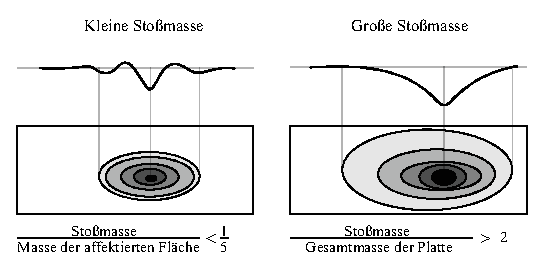
\includegraphics[width=\linewidth]{pictures/einleitung/MassenkriterionOlsson.eps}
	\caption{Massenkriterion nach Olsson}	
	\label{fig:Olsson}
\end{figure}


Zuletzt wollen wir noch auf das Kriterion für mittlere Stoßmassen eingehen. Bei einem zentriertem Stoß auf einer quasi-isotropischen Platte ergibt sich:

\begin{equation}
	\frac{1}{5} < \frac{M}{M_{pmax}} < 2
\end{equation}

Da dieser jedoch für diese Arbeit nicht von großer Relevanz ist, wird hier nicht näher darauf eingegangen.



Im Rahmen der Stoßversuche werden in der aktuellen Forschung vor allem
Untersuchungen mit Laminatverbundsplatten durchgeführt. [Olsson etc]. Hierbei
konzentriert sich ein Großteil der Forschung auf Stöße in der Plattenmitte
[Olsson, Shivakumar etc]. \\
Um das Plattenverhalten während und nach des Stoßes zu beschreiben, wird unter
anderem auf Energie-Masse und Feder-Masse Modelle die von Shivakumar et al.
aufgestellt wurden zurückgegriffen. [Shivakumar] \\
Weitere Modelle wurden von Karas und Olsson hergeleitet, wobei das Modell von
Karas einen Hauptbestandteil dieser Arbeit darstellt. [CITATION NEEDED] Olsson
befasst sich in seiner Arbeit vor allem mit Verbundlaminaten und Delamination
aufgrund von Stößen. \\
Andererseits stellt Karas in seiner Arbeit eine Berechnungsgrundlage für
Stoßvorgänge mit Navierschen Randbedingungen [Vielleicht kurz erklären?] und
einer reduzierten Plattenmasse dar. Die Berechnungen und physikalischen
Grundlagen werden im Theorieteil dieser Arbeit genauer erklärt, weshalb diese
hier nicht weiter vertieft werden.\\
Eine weitere Berechnungsmethode wurde von Reissner und Mindlin entworfen. Diese
ist auch gütlig, wenn die Kirchoff'sche Plattenbedingung nicht anwendbar ist:
\begin{equation}
\frac{Plattendicke}{Seitenl\ddot{a}nge} = \frac{1}{10}
\end{equation}
In der sogenannten Reissner-Mindlin Plattentheorie wird angenommen, dass die
Plattennormale während Deformation nicht orthogonal zur Plattenmittelebene
bleibt. Hierdurch eignet sich diese auch zur Berechnung von
Schubspannungseffekten. [Onate]\\
Da die Berechnung nach Reissner-Mindlin das lösen von Differentialgleichungen
höherer Ordnung erfordert, stellt sie für diese Arbeit nur einen geringen Anteil
dar und wird daher bei Bedarf genauer erläutert. [satz evtl entfernen]\\




		\cleardoublepage
	\chapter{Theoretischer Lösungsansatz}
\label{chap:Principles}

Der Stoßvorgang besteht im Wesentlichen aus einer Kugel mit einem vorgeschriebenen Gewicht $m_g$ welche auf eine reckteckige Platte stößt. Hierbei ist die Auftreffgeschwindigkeit bekannt so wie alle Größen in Tabelle~\ref{tab:TheorieVariablen}. Der Indize "g" bei der Masse der Kugel kommt aus der Literatur nach Karas~\cite{Karas.1939}, wo "g" für Gewicht steht. 

\begin{table}[h!]
	\begin{center}
		\caption{Bekannte Größen während des Stoßvorganges}
		\label{tab:TheorieVariablen}
		
		\begin{tabular}[h]{l | l}	
			Formelzeichen & Beschreibung \\
			\hline
			%$w(x,y,t)$ & Durchbiegung der Platte \\
			%$v(t)$ & Geschwindigkeit der Kugel\\
			%$u(t)$ & Ort des stoßendes Körpers \\
			$m_g$ & Masse der Kugel \\
			$\rho_p$ & Dichte der Platte\\
			$a$ & Breite der Platte\\
			$b$ & Länge der Platte\\
			$h$ & Dicke der Platte \\
			$E$ & E-Modul der Platte \\
			$\nu$ & Poissonzahl der Platte \\
			$\xi$ & x-Koordinate des Auftreffpunktes der Kugel \\
			$\eta$ & y-Koordinate des Auftreffpunktes der Kugel \\
		\end{tabular}
		
	\end{center}
\end{table}


Es wird angenommen, dass der Stoß völlig elastisch verläuft sowie, dass weder die Masse der Kugel, noch die Masse der Platte sich während des Stoßes verändert.
Zusätzlich wird davon ausgegangen, dass der Geschwindigkeitsvektor der Kugel senkrecht zur Platte bzw. parallel zur Normalen liegt. Im Gegensatz zu vielen wissenschaftlichen Arbeiten wird von einem isotropen Material ausgegangen. Somit gelten die im folgenden beschrieben Ergebnisse nur bedingt für Laminate, Faserverbundstoffe oder ähnliche nicht-isotrope Materialien. 

%Desweiteren wird angenommen, dass der dynamische Biegungspfeil an der Stoßstelle %genau so groß ist, wie der statische Biegungspfeil also wenn die Masse $m_g$ %genau an jener Stelle auf die Platte gelegt wird.

Die Annahme, dass Schubspannungen vernachlässigt werden können erlaubt eine geschlossene analytische Lösung des Problems unter der Bedingung, dass die Ränder frei gelagert sind. Somit treten lediglich Biegemomente und keine Schubkräfte auf.

Im folgenden wird die Durchbiegung der Platte als $w(x,y)$ bezeichnet. Die Last $q(x,y)$ wird ebenfalls als ortsabhängige Funktion ausgedrückt. 
Es gilt die allgemeine Differentialgleichung für die Biegung einer Platte unter einer Last $q$, die im Folgenden als bekannt angenommen wird mit $ \nabla = \left(\frac{\partial}{\partial x} \ \frac{\partial}{\partial y} \right)^T$
\begin{equation}
	D \nabla^4 w = q
\label{eq:dgl}
\end{equation}

Die Plattensteifigkeit $D$ errechnet sich aus dem E-Modul und der Poissonzahl $\nu$ wie folgt:
\begin{equation}
D = \dfrac{E h^3}{12 (1-\nu^2)}
\label{eq:D}
\end{equation}


\section{Lösung der Differentialgleichung mit dem Ansatz von Navier}

\begin{figure}[hbt!]
\centering
\begin{overpic}[scale=0.5]{pictures/theory/theory1.eps}
	\put (90,80) {$x$}
	\put (30,10) {$y$}
	\put (40,79) {$\xi$}
	\put (18,60) {$\eta$}
	\put (50,90) {$a$}
	\put (5,45)  {$b$}
	\put (56,27) {$u$}
	\put (75,45)  {$v$}
\end{overpic}

\caption{Stoßfläche auf der Platte}
\label{fig:platte1}
\end{figure}






Navier hat eine Lösung für Gleichung \ref{eq:dgl} unter der Bedingung einer freien Lagerung an den Rändern gezeigt. Dies bedeutet:

\begin{align}
 \tag{x = 0,a \quad y = 0,b}w(x,y) = \Delta w(x,y) = 0	
\end{align}

Er drückt hierfür die unbekannte Durchbiegung der Platte $w(x,y)$ so wie die Last $q(x,y)$ als Reihenausdrücke aus mit $m,n = 1,2,3,4...$:

\begin{equation} 
w(x,y) = \sum_m \sum_n A_{mn} \cdot \sin\left(\dfrac{m \pi x}{a}\right) \cdot \sin\left(\dfrac{n \pi y}{b}\right)
\label{eq:wxy}
\end{equation} 

\begin{equation} 
q(x,y) = \sum_m \sum_n B_{mn} \cdot \sin\left(\dfrac{m \pi x}{a}\right) \cdot \sin\left(\dfrac{n \pi y}{b}\right)
\label{eq:qxy}
\end{equation} 

Man sieht leicht, dass für $x=0,a$ und $y=0,b$ die Randbedingungen direkt erfüllt sind.

Um $B_{mn}$ zu bestimmen, wird nach Timoshenko~\cite{Timoshenko.1922} und Mingyu~\cite{Mingyu.2019} Gleichung \ref{eq:qxy} zunächst mit $\sin{\left( \frac{i \pi x}{a}\right)}$ erweitert und anschließend von $0$ bis $a$ integriert. Da:

\begin{equation}
	\int_0^a \sin{\left( \frac{m \pi x}{a}\right)} \sin{\left( \frac{i \pi x}{a}\right)} dx = 
	\begin{cases}
	0,&  m\neq i\\
	\frac{a}{2},&   m = i 
	\end{cases}
\end{equation}

Das Ergebnis lautet anschließend:

\begin{equation}
	\int_0^a q(x,y) \sin{\left( \frac{i \pi x}{a}\right)} dx = \frac{a}{2} \sum_{n=1}^\infty B_{mn} \sin{\left( \frac{n \pi y}{b}\right)}
\end{equation}

Wenn ebenfalls mit $\sin{\left( \frac{j \pi y}{b}\right)}$ erweitert wird, ergibt sich:


\begin{equation}
\int_0^a \int_0^b q(x,y) \sin{\left( \frac{i \pi x}{a}\right)} \sin{\left( \frac{j \pi y}{a}\right)} dy dx = \frac{ab}{4}  B_{ij} 
\end{equation}


Da $i$ und $j$ frei gewählt wurden, können Sie durch $m$ und $n$ wieder ersetzt werden, so dass:


\begin{equation}
B_{mn} = \dfrac{4}{ab} \cdot \left( \int_0^a \int_0^b q(x,y) 
\sin\left(\dfrac{m \pi x}{a}\right) \cdot \sin\left( \dfrac{n \pi y}{b}\right) dy dx\right)
\label{eq:Bmn_allgemein}
\end{equation}

$A_{mn}$ ergibt sich durch einsetzen von \ref{eq:wxy} und der bekannten Last in Gleichung \ref{eq:dgl} zu:

\begin{equation}
A_{mn} = \dfrac{B_{mn}}{\pi^4 D \left(\dfrac{m^2}{a^2} + \dfrac{n^2}{b^2} \right)^2}
\label{eq:Amn_aus_Bmn}
\end{equation}

In der Regel wird hier jedoch nicht der Fall betrachtet, dass die Kraft gleichmäßig über die gesamte Fläche angreift, sondern nur in einem kleinem Bereich $(u,v)$ an der Stelle $(\xi, \eta)$. Der Last-Koeffizient $B_{mn}$ vereinfacht sich zu:

\begin{align}
B_{mn} &= \dfrac{4}{ab} \cdot \left( \int_{\xi-u/2}^{\xi+u/2} \int_{\eta - v/2}^{\eta + v/2} \dfrac{P}{u v}
\sin\left(\dfrac{m \pi x}{a}\right) \cdot \sin\left( \dfrac{n \pi y}{b} \right)dy dx\right) \\
&= \dfrac{16P}{\pi^2 m n u v} 
\cdot \sin\left(\dfrac{m \pi \xi}{a}\right) 
\cdot \sin\left(\dfrac{n \pi \eta}{b}\right) 
\cdot \sin\left(\dfrac{m \pi u}{2a}\right) 
\cdot \sin\left(\dfrac{n \pi v}{2b}\right)
\label{eq:Bmn_stelle}
\end{align}

Da im folgenden lediglich die Verformung unter einer Kraft $P$ an der Stelle $(\xi, \eta)$ relevant ist, wird der Grenzfall betrachtet in welchem die Fläche $(u,v)$ gegen 0 strebt. Es ergibt sich unter einer Grenzwertbetrachtung von \ref{eq:Bmn_stelle} direkt:

\begin{equation}
B_{mn} = \dfrac{4P}{a b} 
\cdot \sin\left(\dfrac{m \pi \xi}{a}\right) 
\cdot \sin\left(\dfrac{n \pi \eta}{b}\right) 
\label{eq:Bmn_singular}
\end{equation}

Als statische Durchbiegung der Platte unter der Kraft $P$ an der Stelle $(\xi, \eta)$ ergibt sich folglich durch einsetzen von \ref{eq:Bmn_singular} in \ref{eq:Amn_aus_Bmn}:
 
\begin{equation}
 \mathlarger{
 	w(x,y,\xi,\eta) = \frac{4P}{\pi^4 a b D} 
 	\sum_{m = 1}^{\infty} \sum_{n = 1}^{\infty}
 	\frac{
 		\sin\left(\frac{m \pi \xi}{a}\right) 
 		\cdot \sin\left(\frac{n \pi \eta}{b}\right) 
 	}{
 		\left( 
 		\frac{m^2}{a^2} +
 		\frac{n^2}{b^2}
 		\right)^2
 	}
 	\cdot \sin\left(\frac{m \pi x}{a}\right) 
 	\cdot \sin\left(\frac{n \pi y}{b}\right) 
 }
 \end{equation}
 
Die Absenkung unter dem Druckpunkt ergibt sich somit zu:

\begin{equation}
 \mathlarger{
	w(\xi,\eta) = \frac{4P}{\pi^4 a b D} 
	\sum_{m = 1}^{\infty} \sum_{n = 1}^{\infty}
	\frac{
		\sin\left(\frac{m \pi \xi}{a}\right)^2 
		\cdot 	\sin\left(\frac{n \pi \eta}{b}\right) ^2
	}{
		\left( 
		\frac{m^2}{a^2} +
		\frac{n^2}{b^2}
		\right)^2
	}
}
\end{equation}



\section{Dynamische Durchbiegung unter strenger Betrachtung}

Da der zuvor beschriebene Ansatz keinen Aufschluss über das zeitliche Verhalten liefert, wird eine strenge Betrachtung der Durchbiegung erläutert. Hierfür werden die potentiellen und kinetischen Energien in die Lagrange-Gleichung 2. Ordnung eingeführt.

\subsection{Kinetische Energie der Platte}

Die kinetische Energie ergibt sich durch Verallgemeinerung von $T = \frac{1}{2} mv^2$ zu:

\begin{equation}
T = \dfrac{\rho h}{2} \int_{0}^{a} \int_{0}^{b} \left(\dfrac{d}{dt} w(x)\right)^2 dy \ dx
\end{equation}

Da im dynamischen Fall die Durchbiegung der Platte $w(x,y,t)$ eine Zeitabhängigkeit aufweist, wird direkt ersichtlich, dass $A_{mn}$ ebenfalls eine Zeitabhängigkeit aufweisen muss. Somit vereinfachert sich der Differentialausdruck wie folgt:

%Wenn man (2.3) in (2.12) unter Voraussetzung des dynamischen Falls, in dem $A_{mn} = f(Zeit)$ gilt, einsetzt, erhält man direkt: 

\begin{align}
\begin{split}
T &= \dfrac{1}{2}\rho h \int_0^a \int_0^b  \left[\dfrac{d}{dt} \sum_m \sum_n A_{mn} \cdot \sin\left(\dfrac{m \pi x}{a}\right) \cdot \sin\left(\dfrac{n \pi y}{b}\right) \right]^2 dy \ dx  \\
&= \dfrac{1}{2} \rho h\int_0^a \int_0^b  \left[ \sum_m \sum_n \dfrac{d}{dt}\left(A_{mn}\right) \cdot \sin\left(\dfrac{m \pi x}{a}\right) \cdot \sin\left(\dfrac{n \pi y}{b}\right) \right]^2 dy \ dx \\
&= \dfrac{1}{2} \rho h \int_0^a \int_0^b  \left[ \sum_m \sum_n \dot{A}_{mn} \cdot \sin\left(\dfrac{m \pi x}{a}\right) \cdot \sin\left(\dfrac{n \pi y}{b}\right) \right]^2 dy \ dx \\
\end{split}
\label{eq:T_general}
\end{align}

Zum Lösen des Integrals, muss zunächst das Quadrat aufgelöst werden. Zur Vereinfacherung wird einer ganzen Zahl $q$ ein Zahlenpaar $(m,n)$ zugewiesen.
Somit lässt sich die doppelte Summe wie folgt ausdrücken:

$$\sum_m\sum_n K_{mn}=\sum_q K_q$$

Es folgt leicht, dass:

$$\left(\sum_qA_q\right)^2=\sum_qA^2_q+2\sum_q\sum_{p\neq q}A_qA_p$$


Angewendet auf Gleichung \ref{eq:T_general}, erhält man für die quadratischen Terme:

\begin{equation}
\dfrac{1}{2}\rho h \sum_m\sum_n \dot{A}^2_{mn}\int_0^a\sin^2\left(\dfrac{m\pi x}{a}\right)\int_0^b\sin^2\left(\dfrac{n\pi y}{b}\right) dy \ dx=\dfrac{1}{8}\rho h a b\sum_m\sum_n \dot{A}^2_{mn}
\end{equation}

\newpage

Die doppelte Summe über $(p,q)$ wird als vierfache Summe wie folgt ausgedrückt:



\begin{equation}
\dfrac{1}{2}\rho h \sum_m\sum_n\sum_i\sum_j \dot{A}_{mn}\dot{A}_{ij}\int_0^a\sin\left(\dfrac{m\pi x}{a}\right)\sin\left(\dfrac{i\pi x}{a}\right)\int_0^b\sin\left(\dfrac{n\pi y}{b}\right)\sin\left(\dfrac{j\pi y}{b}\right) dy \ dx
\end{equation}

Unter genauer Betrachtung fällt auf, dass $m\neq i$ oder $n\neq j$ da $q\neq p$. Dies führt dazu, dass stehts mindestens eins der beiden Integrale sich zu null ergibt. Somit folgt für die kinetische Energie:

\begin{equation}
T = \dfrac{1}{8}\rho h a b\sum_m\sum_n \dot{A}^2_{mn}
\label{eq:T}
\end{equation}



%-----------------------------------------------------------------------------------------------------------------------
% 											V E R Z E R R U N G S E N E R G I E
%-----------------------------------------------------------------------------------------------------------------------






\subsection{Verzerrungsenergie durch Dehnung aufgrund von Biegung und Torsion}

Unter der Annahme, dass die Platte nur durch ein Moment $M_y \cdot \Delta y$ um einen Winkel $\theta$ um die y-Achse verbogen wird , berechnet sich die Verzerrungsenergie zunächst durch: $$\Delta U = \frac{1}{2} (M_y \cdot \Delta y) \cdot \theta$$. 

\begin{center}
	\begin{overpic}[scale=0.3]{pictures/theory/theory2.eps}
		\put (47,75) {$\displaystyle\theta$}
		\put (15,60) {$R$}
		\put (45,20) {$\Delta x$}
	\end{overpic}
	
\end{center}

Der Krümmungsradius $R$ kann wie folgt durch die Durchbiegung ausgedrückt werden: $R^{-1} = \frac{\partial^2 w}{\partial x^2}$. Mit $\Delta x = R \cdot \theta$ folgt direkt:

\begin{equation}
\Delta U = \dfrac{1}{2}(M_y \Delta y) \dfrac{\partial^2 w}{\partial x^2} \Delta x
\label{eq:dU_d}
\end{equation}

Wenn ebenfalls $M_{xy}$ und $M_x$ mit einbezogen werden, ergibt sich Gleichung \ref{eq:dU_d} zu:

\begin{equation}
\Delta U = \dfrac{1}{2}\left( M_y  \dfrac{\partial^2 w}{\partial x^2} + M_x  \dfrac{\partial^2 w}{\partial y^2} - 2 \cdot M_{xy}\dfrac{\partial^2 w}{\partial x \partial y} \right) \Delta x \Delta y
\end{equation}

Die unbekannten Momente können wiederum durch die Plattensteifigkeit und Krümmung der Platte ausgedrückt werden. Somit ergibt sich:

\begin{align}
\begin{split}
\Delta U 	&=  \dfrac{D}{2}\left[
\left(\dfrac{\partial^2 w}{\partial x^2}\right)^2
+ 2 \nu \dfrac{\partial^2 w}{\partial x^2} \dfrac{\partial^2 w}{\partial y^2}
+ 2(1-\nu) \left(\dfrac{\partial^2 w}{\partial x \partial y}\right)^2
+ \left(\dfrac{\partial^2 w}{\partial y^2}\right)^2 \right] \Delta x \Delta y\\
&=  \dfrac{D}{2}\left[
\left(
\dfrac{\partial^2 w}{\partial x^2} + \dfrac{\partial^2 w}{\partial y^2}\right)^2 
- 2 (1-\nu) \left( \dfrac{\partial^2 w}{\partial x^2} \dfrac{\partial^2 w}{\partial y^2} - \left( \dfrac{\partial^2 w}{\partial x \partial y} \right)^2\right) \right] \Delta x \Delta y\\
\end{split}
\label{eq:dU_ddd}
\end{align}


Durch Einsetzen von \ref{eq:wxy} in \ref{eq:dU_ddd} und einer anschließenden Integration über die Platte ergibt sich die potentielle Energie zu:


\begin{multline}
U = \int_0^a \int_0^b \left\{
\frac{D}{2} \sum_{m = 1}^{\infty}\sum_{n = 1}^{\infty} A^2_{mn}
\left[
\pi^4 \left(\frac{m^2}{a^2} + \frac{n^2}{b^2}\right)^2
\sin^2\left(\frac{m\pi x}{a}\right) \sin^2\left(\frac{n\pi y}{b}\right)
\right.
\right. \\
\left.
\left.
-2(1-\nu) 
\frac{m^2n^2\pi^4}{a^2b^2}
\left(
\sin^2\left(\frac{m\pi x}{a}\right) 
\sin^2\left(\frac{n\pi y}{b}\right)
- 
\cos^2\left(\frac{m\pi x}{a}\right) 
\cos^2\left(\frac{n\pi y}{b}\right)
\right)
\right] 
\right\}
\end{multline}

Das Ergebnis der Integration lautet:

\begin{equation}
U = \dfrac{D \cdot a b \cdot \pi^4}{8} \sum_{m=1}^{\infty}  \sum_{n=1}^{\infty} A^2_{mn}  \left( \dfrac{m^2}{a^2} + \dfrac{n^2}{b^2}\right)^2
\label{eq:U}
\end{equation}

\subsection{Einsetzen in die Lagrange Gleichung}

Da in \ref{eq:U} nicht die verrichtete Arbeit der angreifenden Kraft $P$ berücksichtigt wurde, ergibt sich in der Lagrangegleichung eine Konstante $Q_{mn}$ welche zu einem späteren Zeitpunkt bestimmt wird.

\begin{equation}
\dfrac{d}{dt} \dfrac{\partial T}{\partial \dot{A}_{mn}} - \dfrac{\partial T}{\partial A_{mn}} + \dfrac{\partial U}{\partial A_{mn}} = Q_{mn}
\end{equation}

Durch einsetzen von \ref{eq:U} und \ref{eq:T} folgt direkt:

\begin{equation}
\ddot{A}_{mn} + \left(\dfrac{m^2}{a^2} + \dfrac{n^2}{b^2}\right)^2 \pi^4 \overline{a}^2 A_{mn} = \dfrac{4}{\rho h a b} Q_{mn}
\label{eq:lagrangeDGL}
\end{equation}

\newpage

mit dem Faktor $\overline{a}$ gegeben durch \ref{eq:aquer}.


\begin{equation}\overline{a} = \sqrt{\dfrac{D}{\rho h}} = \sqrt{\dfrac{E h^2}{12 \rho (1-\nu^2)}}
\label{eq:aquer}
\end{equation}

Durch Integration von \ref{eq:lagrangeDGL} und unter Berücksichtigung der zeitlichen Randbeding $A_{mn} = \dot{A}_{mn} = 0 \text{ für } t = 0$ fallen nach Karas~\cite{Karas.1939} die Integrationskonstanten weg, so dass $A_{mn}$ wie folgt ausgerechnet werden kann:

\begin{equation}
A_{mn} = \dfrac{1}{\pi^2 \overline{a}  \left(\frac{m^2}{a^2} + \frac{n^2}{b^2} \right)} \dfrac{4}{\rho h a b} \int_0^t	Q_{mn}(\tau) \sin \left[ \left(\frac{m^2}{a^2} + \frac{n^2}{b^2} \right) \pi^2 \overline{a} (t-\tau)\right] d\tau
\label{eq:Amn_full}
\end{equation}


Die wirkende Kraft die der Körper auf die Platte ausübt sei nun als $P(\tau)$ bezeichnet. 
Da angenommen wird, dass die Kraft punktuell an der Stelle $(\xi, \eta)$ angreift, folgt für die virtuelle Arbeit $\delta E$ von $P$

\begin{equation}
\delta E = P \delta A_{mn} \cdot \sin \left( \frac{m \pi \xi}{a} \right) \sin \left( \frac{n \pi \eta}{b} \right) = Q_{mn} \cdot \delta A_{mn}
\end{equation} 

es folgt:

\begin{equation}
Q_{mn}(\tau) = P(\tau) \sin \left( \frac{m \pi \xi}{a} \right) \sin \left( \frac{n \pi \eta}{b} \right)
\label{eq_Qmntau}
\end{equation}



Wenn nun schließlich Gleichung \ref{eq_Qmntau} in Gleichung \ref{eq:Amn_full} eingesetzt wird, welche wiederum in Gleichung \ref{eq:wxy} eingesetzt wird, ergibt sich die Durchbiegung als Abhängigkeit des Stoßgewichtes $P(\tau)$ und der Zeit.

\begin{multline}
w(x,y,\xi, \eta, t) = \sum_m \sum_n 
\dfrac{1}{\pi^2 \overline{a}  \left(\frac{m^2}{a^2} + \frac{n^2}{b^2} \right)} \dfrac{4}{\rho h a b} \\ \int_0^t
 P(\tau) \sin \left( \frac{m \pi \xi}{a} \right) \sin \left( \frac{n \pi \eta}{b} \right)
\sin \left[ \left(\frac{m^2}{a^2} + \frac{n^2}{b^2} \right) \pi^2 \overline{a} (t-\tau)\right] d\tau
\cdot \sin\left(\frac{m \pi x}{a}\right) \cdot \sin\left(\frac{n \pi y}{b}\right)
\end{multline}

\newpage

Umgeschrieben ergibt sich:

\begin{multline}
	w(x,y,\xi, \eta, t) = \dfrac{4}{\rho h a b \pi^2 \overline{a}} \cdot \sum_m \sum_n 
	\dfrac{\sin\left(\frac{m \pi x}{a}\right) \cdot \sin\left(\frac{n \pi y}{b}\right) \sin\left(\frac{m \pi \xi}{a}\right) \cdot \sin\left(\frac{n \pi \eta}{b}\right)	}{\left(\frac{m^2}{a^2} + \frac{n^2}{b^2} \right)}  \\
	\int_0^t
	P(\tau)\cdot \sin \left[ \left(\frac{m^2}{a^2} + \frac{n^2}{b^2} \right) \pi^2 \overline{a} (t-\tau)\right] d\tau
	\label{eq:wxyxietat}
\end{multline}


Die einzige Unbekannte in der Gleichung ist nun die Stoßkraft $P(\tau)$. Da im Allgemeinen die Stoßkraft in Abhängigkeit von der Zeit nicht gegeben ist, wird im folgenden die Stoßkraft in Abhängigkeit des Eindringunsweges des stoßendes Körpers in die Platte verwendet. Wenn nun der Eindringungsweg als $z$ bezeichnet wird sowie die Position des stoßendes Körper gegen den ruhenden Raum als $u$, ergibt sich direkt:

\begin{equation}
	u = z + w
\end{equation}


Durch Integration des zweiten Newton'schen Axioms, mit der Masse $m_g$ des stoßendes Körpers, ergibt sich für die Geschwindigkeit 

\begin{equation}
	v = v_0 - \frac{1}{m_g} \int_0^t P(\tau) d\tau
	\label{eq:speedEq}
\end{equation}

Durch Integration ergibt sich folglich für den Ort des stoßendes Körpers:

\begin{equation}
	u = v_0 \cdot t - \frac{1}{m_g} \int_0^t P(\tau) (t-\tau) d\tau
	\label{eq:mpos}
\end{equation}


Da jedoch im Allgemeinen die Kraft in Abhängigkeit vom Eindringungsweg und umgekehrt bekannt ist, wird $z(P)$ im folgenden genutzt:

\newpage

Wenn man nun Gleichung \ref{eq:mpos} mit \ref{eq:wxyxietat} und $z(P)$ zusammenführt, ergibt sich folgender Ausdruck:


\begin{multline}
v_0 \cdot t - \frac{1}{m_g} \int_0^t P(\tau) (t-\tau) d\tau = z(P) + \dfrac{4}{\rho h a b \pi^2 \overline{a}} \cdot  \\  \sum_m \sum_n 
\dfrac{{\sin\left(\frac{m \pi x}{a}\right) \cdot \sin\left(\frac{n \pi y}{b}\right) \sin\left(\frac{m \pi \xi}{a}\right) \cdot \sin\left(\frac{n \pi \eta}{b}\right)	}}{\left(\frac{m^2}{a^2} + \frac{n^2}{b^2} \right)} 
\int_0^t
P(\tau)\cdot \sin \left[ \left(\frac{m^2}{a^2} + \frac{n^2}{b^2} \right) \pi^2 \overline{a} (t-\tau)\right] d\tau
\label{eq:long_solution}
\end{multline}

Im Allgemeinen ist Gleichung \ref{eq:long_solution} nicht oder nur kaum analytisch lösbar. Hingegen kann das Integral numerisch gelöst werden, in dem man das Intervall $\left[ 0,t \right]$ in $\theta$ Teilintervalle der Länge

 \begin{equation}
 	\tau = \dfrac{\mbox{t}}{\theta}=\dfrac{T}{\kappa}
 \end{equation}
 
 unterteilt, worin $T$ die Schwingungsdauer der Platte beschreibt. $\kappa$ muss groß genug gewählt werden, damit numerische Ungenauigkeiten minimal werden. In der Literatur wurde hier entweder $180$ oder $360$ gewählt. Falls die Teilintervalle klein genug sind, kann die Kraft $P(\tau	)$ in jedem Intervall $i$ als zeitlich konstant angenähert werden. Im Intervall $(i-1) \rightarrow i$ ist dann $P_{i}$ der konstante Wert von $P(\tau)$. Desweiteren ergibt sich mit dieser Vereinfacherung das Integral in \ref{eq:long_solution} zu:
 
 \begin{equation}
 	\frac{1}{\pi^2\overline{a}} \cdot \frac{1}{\frac{m^2}{a^2}+\frac{n^2}{b^2}} \cos \left[ \left( \frac{m^2}{a^2}+\frac{n^2}{b^2} \right) \pi^2\overline{a}(\theta - i)\tau\right]
 \end{equation}  
 
Mit:

$$\cos\left(\overline{\theta - i}\right) \coloneqq \cos \left[ \left( \frac{m^2}{a^2}+\frac{n^2}{b^2} \right) \pi^2\overline{a}(\theta - i)\tau\right] $$

\newpage

folgt für die Lösung:

\begin{equation}
\begin{multlined}
	w(x,y,\xi, \eta) = \frac{4}{\rho h a b \pi^4 \overline{a}^2} \cdot \left[ P_{1} \sum_m \sum_n \frac{\sin\left(\frac{m \pi x}{a}\right) \cdot \sin\left(\frac{n \pi y}{b}\right) \sin\left(\frac{m \pi \xi}{a}\right) \cdot \sin\left(\frac{n \pi \eta}{b}\right)	}{ \left( \frac{m^2}{a^2} + \frac{n^2}{b^2} \right)^2} \cdot \left( \cos(\overline{\theta-1}) - \cos(\overline{\theta}) \right) + \right. \\ P_{2} \sum_m \sum_n \frac{\sin\left(\frac{m \pi x}{a}\right) \cdot \sin\left(\frac{n \pi y}{b}\right) \sin\left(\frac{m \pi \xi}{a}\right) \cdot \sin\left(\frac{n \pi \eta}{b}\right)	}{ \left( \frac{m^2}{a^2} + \frac{n^2}{b^2} \right)^2} \cdot \left( \cos(\overline{\theta-2}) - \cos(\overline{\theta-1}) \right) + . \; . \; .\ \\ \left. + P_{\theta} \sum_m \sum_n \frac{\sin\left(\frac{m \pi x}{a}\right) \cdot \sin\left(\frac{n \pi y}{b}\right) \sin\left(\frac{m \pi \xi}{a}\right) \cdot \sin\left(\frac{n \pi \eta}{b}\right)	}{ \left( \frac{m^2}{a^2} + \frac{n^2}{b^2} \right)^2} \cdot \left( 1 - \cos(\overline{1}) \right) \right]
	\label{eq:horror}
\end{multlined}
\end{equation}


beziehungsweise mit $(i=1,2 ... \theta)$: 

\begin{multline}
 	w(x,y,\xi, \eta) = \frac{4}{\rho h a b \pi^4 \overline{a}^2} \sum_i \sum_m \sum_n P_{i} \cdot \\ \frac{\sin\left(\frac{m \pi x}{a}\right) \cdot \sin\left(\frac{n \pi y}{b}\right) \sin\left(\frac{m \pi \xi}{a}\right) \cdot \sin\left(\frac{n \pi \eta}{b}\right)	}{ \left( \frac{m^2}{a^2} + \frac{n^2}{b^2} \right)^2} \left( \cos(\overline{\theta - i}) - \cos(\overline{\theta - (i-1)}) \right) 	
\label{eq:numericalSolution}
\end{multline}

welcher dann statt dem letzten Term in \ref{eq:wxyxietat} eingesetzt wird. $T$ und die Kreisfrequenz $\omega = \frac{2 \pi}{T}$ können direkt aus \ref{eq:lagrangeDGL} abgelesen werden: 

\begin{equation}
	T = \frac{2 \pi}{\pi^2 \overline{a} \left( \frac{1}{a^2} + \frac{1}{b^2} \right) }, \qquad \omega=\pi^2 \overline{a} \left( \frac{1}{a^2}+\frac{1}{b^2} \right)
\end{equation}

Mit einem genügend groß gewähltem $\kappa$, hier $\kappa=180$, kommt man für die Intervalllänge auf

\begin{equation}
	\tau = \frac{\pi}{90} \cdot \frac{1}{\pi^2 \overline{a} \left( \frac{1}{a^2} + \frac{1}{b^2} \right) }
	\label{eq:tau}
\end{equation}

\newpage

Da in \ref{eq:numericalSolution} die doppelten Summe über $m,n$ häufig vorkommen, kann man um Rechenzeit zu sparen, $\overline{S(k)}$ als den Summenausdruck definieren. Mit \ref{eq:tau} und $k=\theta - i$:

\begin{equation}
\begin{split}
\overline{S(k)} & = \sum_m \sum_n \frac{\sin\left(\frac{m \pi x}{a}\right) \cdot \sin\left(\frac{n \pi y}{b}\right) \sin\left(\frac{m \pi \xi}{a}\right) \cdot \sin\left(\frac{n \pi \eta}{b}\right)	}{ \left( \frac{m^2}{a^2} + \frac{n^2}{b^2} \right)^2} \cdot \cos\left(\overline{\theta - i}\right) \\ 
& = \sum_m \sum_n \frac{\sin\left(\frac{m \pi x}{a}\right) \cdot \sin\left(\frac{n \pi y}{b}\right) \sin\left(\frac{m \pi \xi}{a}\right) \cdot \sin\left(\frac{n \pi \eta}{b}\right)	}{ \left( \frac{m^2}{a^2} + \frac{n^2}{b^2} \right)^2} \cdot \cos \left[ \left( \frac{m^2}{a^2}+\frac{n^2}{b^2} \right) \pi^2\overline{a}(\theta - i)\tau\right] \\
&= \sum_m \sum_n \frac{\sin\left(\frac{m \pi x}{a}\right) \cdot \sin\left(\frac{n \pi y}{b}\right) \sin\left(\frac{m \pi \xi}{a}\right) \cdot \sin\left(\frac{n \pi \eta}{b}\right)	}{ \left( \frac{m^2}{a^2} + \frac{n^2}{b^2} \right)^2} \cdot \cos \left[ \left( \frac{m^2}{a^2}+\frac{n^2}{b^2} \right) \frac{\pi k}{90} \cdot \frac{a^{2}b^{2}}{a^{2}+b^{2}} \right] \\
\end{split}
\end{equation}


Anschließend vereinfachert sich \ref{eq:numericalSolution} zu:

\begin{equation}
w(x,y,\xi, \eta) = \frac{4}{\rho h a b \pi^4 \overline{a}^2} \sum_i P_i \cdot (\overline{S(\theta - i)} - \overline{S(\theta - (i-1))})
\end{equation}




			\cleardoublepage
	\chapter{Durchführung}
\label{chap:Durchfuehrung}

In der bereits hergeleiteten Theorie wird der Lösungsweg für das beschrieben Problem vorgestellt. Mit dem zur Verfügung gestelltem Skript, das auf dieser Theorie basiert wird nun die Parameterstudie durchgeführt. Um relevante Ergebnisse zu erlangen, müssen zuerst weitere Gleichungen in das Skript eingearbeitet werden.\\
In dem Skript wird eine Konstante $c$ als Vorfaktor für die Kraftberechnung aus dem Punktkontakt verwendet. Um die Berechnungsmöglichkeiten zu erweitern, wird $c$ nun durch eine Gleichung der Hertz'schen Pressung ersetzt, die wie folgt Hergeleitet wird:\\
Die Gleichung für die Hertz'sche Pressung eines Kugel-Kugel-Punktkontaktes lautet wie in Gleichung~\ref{form:ZvonP}

\begin{equation}
	\label{form:ZvonP}
	z(P) = \left[ \frac{9 P^{2} (1 - \nu^{2})^{2}}{2 E^{2}} \cdot \left( \frac{1}{2 r_{1}} + \frac{1}{2 r_{2}} \right) \right]^{\frac{1}{3}}
\end{equation}

Da einer der beiden Körper eine Platte mit dem Radius $r_{p} = \infty$ ist, folgt durch einsetzen von $r_{p}$ und umstellen nach P:

\begin{equation}
	\label{form:PvonZ}
	P(z) = \sqrt{\frac{4 r_{g}}{9}} \cdot \frac{E}{(1 - \nu^{2})} \cdot z^{\frac{3}{2}}
\end{equation}
	
Hier ist $\frac{E}{(1 - \nu^{2})}$ der reduzierte E-Modul, welcher durch Gleichung~\ref{form:redE} beschrieben wird.

\begin{equation}
	\label{form:redE}
	\frac{E}{(1 - \nu^{2})} = \left( \frac{(1 - \nu_{p}^{2})}{E_{p}} + \frac{(1 - \nu_{g}^{2})}{E_{g}} \right)^{-1}
\end{equation} 

Nun wird $c$ als Vorfaktor von $z^{\frac{3}{2}}$ in Gleichung~\ref{form:PvonZ} definiert, sodass folgt:

\begin{equation}
	\label{form:c}
	c = \sqrt{\frac{4 r_{g}}{9}} \cdot \frac{E}{(1 - \nu^{2})}
\end{equation}

Im Skript wurden Gleichungen~\ref{form:redE} und~\ref{form:c} unter den Konstanten implementiert und die einstellbaren Parameter der Platte und der Impaktor respektive um $E_{p}$ und $\nu_{p}$, bzw. $E_{g}$ und $\nu_{g}$ erweitert.\\

\section{Vorgehen und Vorbereitung}

Insgesamt wird das Problem durch die einstellbaren Parameter in Tabelle~\ref{tab:VariablenderStudie} beschrieben. In Anlehnung an \cite{Olsson.2000} wird das Massenverhältnis $Mr$ als einer der signifikanten Parameter gewählt. Davon ausgehend werden dann die anderen Parameter einzeln variiert und die Ergebnisse grafisch ausgewertet. 

\begin{table}[H]
	\begin{center}
		\caption{Variablen der Parameterstudie}
		\label{tab:VariablenderStudie}
		\begin{tabular}{l|c}
			\textbf{Variable} & \textbf{Bedeutung}\\
			\hline
			$a,b,h$ & Plattenmaße in [cm]\\
			$r_{g}$ & Impaktorradius in [cm]\\
			$v_{0}$ & Auftreffgeschwindigkeit [cm/s]\\
			$Mr$ & Massenverhältnis $\hat{=}$ $\frac{Impaktormasse}{Plattenmasse}$\\
			$\xi,\eta$ & Auftreffstelle des Impaktors\\
			$x,y$ & Auswertungsstelle\\		
		\end{tabular}
	\end{center}
\end{table}

\subsection{Auswertungskriterien und Annahmen}

Als Auswertungskriterien werden die Anzahl der einzelnen Schläge und der maximal auftretenden Kraft zusammen mit der Auslenkung der Platte gewählt. \\
Für die Studie werden folgende übergreifende Annahmen getroffen: 

\begin{enumerate}
	\item{Die Platte und der Impaktor sind isotrop, mit konstanten Stoffwerten}
	\item{Die Platte und der Impaktor sind aus identischem Material, mit gleichem E-Modul und Poissonzahl $\nu$}
\end{enumerate}

\subsubsection{Anzahl der Schläge}

Als Schlag wird hier ein Kraftverlauf bezeichnet, bei dem die Kraft $P_{i}$ zwischen den Schlägen auf Null fällt, nach der Bedingung in Gleichung~\ref{form:Schlagauftreten}:

\begin{equation} 
	\label{form:Schlagauftreten}
	F_{i-1} > 0 \; \wedge \; F_{i} = 0.0 
\end{equation}

Da im zeitlichen Verlauf auch nach dem ersten Auftreffen noch Schläge auftreten können, wird die Schrittanzahl auf $i = 1000$ gesetzt um signifikante Ergebnisse zu erlangen. 

\subsubsection{Maximale Auslenkung der Platte}

Die maximale Auslenkung $w_{max}$ wird direkt aus der Versuchsreihe ausgelesen und in Abhängigkeit des Massenverhältnisses und des zu veränderten Parameters dargestellt.

\subsubsection{Maximale Kraft}

Analog zur maximalen Auslenkung, wird die maximale Kraft $P_{max}$ direkt ausgelesen und in Abhängigkeit von $Mr$ und dem Parameter dargestellt.



\section{Parameterstudie}

Für die Parameterstudie wurde folgender Fall aus Ausgangspunkt gewählt: 

\begin{table}[H]
	\begin{center}
		\caption{Ausgangsfall Parameterstudie}
		\label{tab:Ausgang}
		\begin{tabular}{l|c}
			\textbf{Variable} & \textbf{Wert}\\
			\hline
			$a$ & 50.0 [cm]\\
			$b$ & 50.0 [cm]\\
			$h$ & 1.0 [cm]\\
			$r_{g}$ & 1.0 [cm]\\
			$v_{0}$ & 500.0 [cm/s]\\
			$\xi,\eta$ & 25.0 [cm]\\
			$x,y$ & 25.0 [cm]\\ 		
		\end{tabular}
	\end{center}
\end{table}

$Mr$ wird hier bewusst ausgelassen, da bei jedem Parameter außer der Auftreffstelle über das Massenverhältnis iteriert wird und dadurch kein Anfangswert, sondern eine Menge benötigt wird. Die Menge der $Mr$ ist nach Gleichung~\ref{form:Mr}:

\begin{equation}
	\label{form:Mr}
	0.01 \leq Mr \leq 2.50 \; , \;\; \mbox{Schrittweite:} \; \Delta Mr = 0.01
\end{equation}

Die Stoffparameter sind im Rahmen der Studie konstant und in Tabelle~\ref{tab:Stoff} definiert.

\begin{table}[H]
	\begin{center}
		\caption{Stoffparameter: Kugel und Platte}
		\label{tab:Stoff}
		\begin{tabular}{l|c}
			\textbf{Variable} & \textbf{Wert}\\
			\hline
			$E_{p}$ & $2.2 \cdot 1e06$ [$kg/cm^2$]\\
			$\nu_{p}$ & 0.3 [-]\\
			$\rho_{p}$ & 0.00796 [$kg/cm^{3}$]\\
			\hline
			$E_{g}$ &  $2.2 \cdot 1e06$ [$kg/cm^2$]\\
			$\nu_{g}$ & 0.3 [-]\\		
		\end{tabular}
	\end{center}
\end{table}

\subsection{Höhe der Platte}

Als erster Parameter wird die Höhe nach Gleichung~\ref{form:DeltaH} variiert. Alle anderen Werte werden nach Tabelle~\ref{tab:Ausgang} konstant gehalten.

\begin{equation}
	\label{form:DeltaH}
	0.5 [cm] \leq h \leq 2.5 [cm], \; \; \mbox{Schrittweite:} \; \Delta h = 0.1 [cm]
\end{equation}

Wenn man die Höhe, das Massenverhältnis und die Anzahl der Schläge aufträgt, ergibt sich Abbildung~\ref{fig:Hoehe}.

\begin{figure}[H]
	\begin{center}
		\begin{overpic}[width=\linewidth]{pictures/gnuplot/3d/Hoehe/production/Hoehe.eps}
			\put(45,4){Höhe [cm]}
			\put(18,30){\rotatebox{90}{Mr [-]}}
			\put(83,60){Aufschläge [-]}
		\end{overpic}
	\caption{Höhe, Mr und Anzahl der Aufschläge}
	\label{fig:Hoehe}
	\end{center}
\end{figure}

Man kann direkt ablesen, dass mehrere Aufschläge vermehrt im unteren Höhenbereich auftreten. Dies ist direkt auf die Steifigkeit der Platte zurückzuführen. Bei größerer Plattendicke ist die Steifigkeit der Platte größer und die Kugel prallt ab, ohne vermehrt aufzutreffen. Bei $h = 0.6 [cm]$ treten bis zu 10 Schlägen auf. Interessant ist auch, dass sich drei Bereiche in Abhängigkeit des Massenverhältnisses ausbilden. \\
Es ist offensichtlich, dass bei einem Massenverhältnis $Mr \geq 1.7$ und einer Plattendicke von $h \geq 1.6 [cm]$ nur noch einzelne Stöße auftreten. Hier ist anzunehmen, dass der elastische Stoßvorgang der Kugel ausreichend kinetische Energie entgegen der Stoßrichtung überträgt, dass sie sich schneller entfernt, als die Platte auslenken kann. \\
Auch bei der Auslenkung stimmen die Ergebnisse mit den Erwartungen überein. In Abbildung~\ref{fig:HoeheAuslenkung} ist zu erkennen, dass mit zunehmender Höhe die Auslenkung abfällt, da die Steifigkeit der Platte zunimmt. Die Steigung der Auslenkungskurve flacht mit zunehmendem $Mr$ ab. Am signifikantestem ist die Steigung im Bereich $0.01 \leq Mr \leq 1$. Ergo ist der Einfluss des Massenverhältnisses am größten in diesem Bereich.\\
Bei Plattendicken von $h \geq 1.3 [cm]$ flacht die Steigung der maximalen Auslenkung in einen annähernd linearen Bereich ab. Daher liegt nahe, dass die Höhe im Bereich bis $h = 1.3 [cm]$ den stärksten Einfluss hat.\\

\begin{figure}[h!]
	\begin{center}
		\begin{overpic}[width=\linewidth]{pictures/gnuplot/3d/Hoehe/production/HoeheAuslenkung.eps}
			\put(45,4){Höhe [cm]}
			\put(18,30){\rotatebox{90}{Mr [-]}}
			\put(83,60){Auslenkung [cm]}
		\end{overpic}
	\caption{Höhe, Mr und Auslenkung}
	\label{fig:HoeheAuslenkung}
	\end{center}
\end{figure}

Die größte Auslenkung tritt bei einem Massenverhältnis von $Mr = 2.5$ und einer Höhe von $h = 0.5 [cm]$ auf und beträgt $w(0.5,2.5) = 2.265 [cm]$, während die geringste Auslenkung bei $Mr = 0.01$ und $h = 2.5 [cm]$ mit $w = 0.0165 [cm]$ auftritt.\\
\\
Wenn man die maximal auftretende Kraft betrachtet, ergibt sich Abbildung~\ref{fig:HoeheKraft}.\\
Aus der maximalen Auslenkung kann man schlussfolgern, dass die maximale Kraft dort auftritt, wo die Auslenkung am geringsten ist, da hier am wenigsten Energie in die Deformation der Platte übergeht.\\
Bei $Mr = 2.5$ und $h = 2.5 [cm]$ tritt daher eine Kraft von $P = 598.36 [kN]$ auf. Die hier auftretende Kraft ist etwa um den Faktor $50$ größer als die geringste Kraft, die wie zu erwarten bei $Mr = 0.01$ und $h = 0.5 [cm]$ auftritt und $P = 10.88 [kN]$ beträgt. \\
Interessant zu betrachten ist auch, wie die Kraft mit größer werdendem $Mr$ zunimmt. Bei $h_{min} = 0.5 [cm]$ ist die Kraft bei $Mr_{max} = 2.5$ nur um den Faktor 2 größer als bei $Mr_{min} = 0.01$. Betrachtet man allerdings $h_{max} = 2.5 [cm]$, ist die Kraft bei $Mr_{max} = 2.5$ um den Faktor $14.4$ größer als bei $Mr_{min} = 0.01$, bzw. betragen die Kräfte $P_{max}(h_{max}) = 598.36[kN]$ und $P_{min}(h_{max}) = 41.4[kN]$.

\begin{figure}[H]
	\begin{center}
		\begin{overpic}[width=\linewidth]{pictures/gnuplot/3d/Hoehe/production/HoeheKraft.eps}
			\put(45,4){Höhe [cm]}
			\put(18,30){\rotatebox{90}{Mr [-]}}
			\put(80,62){Kraft [N]}
		\end{overpic}
	\caption{Höhe, Mr und Kraft}
	\label{fig:HoeheKraft}
	\end{center}
\end{figure}



\subsection{Geschwindigkeit des Impaktors}

Als nächster Parameter wird die Geschwindigkeit betrachtet. Da hier nur der Low-Velocity Bereich betrachtet wird, wird die Geschwindigkeit nach Gleichung~\ref{form:DeltaV0} variiert. 

\begin{equation}
	100 [cm/s] \leq v_{0} \leq 1000 [cm/s] \; , \;\; \mbox{Schrittweite:} \; \Delta v_{0} = 10 [cm/s]
	\label{form:DeltaV0}
\end{equation}

Analog zur Höhenvariation wird zuerst die Anzahl der Aufschläge aufgetragen. In Abbildung~\ref{fig:Speed} ist zu erkennen, dass die Geschwindigkeit bei gleichbleibendem $Mr$ keinen Einfluss auf die Anzahl der Aufschläge hat. 

\begin{figure}[h!]
	\begin{center}
		\begin{overpic}[width=\linewidth]{pictures/gnuplot/3d/Speed/production/Speed.eps}
			\put(40,4){Geschwindigkeit [cm/s]}
			\put(18,30){\rotatebox{90}{Mr [-]}}
			\put(83,60){Aufschläge [-]}
		\end{overpic}
		\caption{Geschwindigkeit, Mr und Anzahl der Aufschläge}
		\label{fig:Speed}
	\end{center}
\end{figure}

Die aus den Stößen resultierende Auslenkung wird in Abbildung~\ref{fig:SpeedAuslenkung} dargestellt. Man kann erkennen, dass der Einfluss des Massenverhältnisses mit zunehmender Geschwindigkeit zunimmt. \\
Die geringste Auslenkung tritt bei $Mr = 0.01$ und $v_{0} = 100 [cm/s]$ auf und beträgt $w = 0.008899 [cm]$, während die größte Auslenkung wie zu erwarten bei $v_{0,max} = 1000 [cm/s]$ und $Mr_{max} = 2.5$ berechnet wird und $w_{max} = 2.57 [cm]$ beträgt. \\
Auch zu sehen ist, dass im höheren Geschwindigkeitsbereich die Auslenkung stärker mit größer werdendem $Mr$ ansteigt. \\
Betrachtet man den Faktor der zwischen der $w_{min}(v_{0,min})$ und $w_{max}(v_{0,max})$ bei gegebenem $Mr$ liegt ist zu erkennen, dass die Geschwindigkeit im Zusammenspiel mit $Mr$ einen großen Einfluss auf die Auslenkung hat. Bei $v_{0,min}$ ist der Faktor mit $28.72$ fast gleich wie bei $v_{0,max}$ mit $29.72$.

\begin{figure}[H]
	\begin{center}
		\begin{overpic}[width=\linewidth]{pictures/gnuplot/3d/Speed/production/SpeedAuslenkung.eps}
			\put(44,4){Geschwindigkeit [cm/s]}
			\put(18,30){\rotatebox{90}{Mr [-]}}
			\put(83,60){Auslenkung [cm]}
		\end{overpic}
		\caption{Geschwindigkeit, Mr und Auslenkung}
		\label{fig:SpeedAuslenkung}
	\end{center}
\end{figure}

Als letztes wird nun die Kraft aufgetragen. In Abbildung~\ref{fig:SpeedKraft} sind ähnliche Trends wie in Abbildung~\ref{fig:SpeedAuslenkung} zu sehen. \\
Auch hier nimmt die auftretende Kraft mit $v_{0}$ zu. Je größer $Mr$ hierbei ist, desto steiler die Kraftzunahme. Besonders deutlich wird dies, wenn man wieder die Faktoren zwischen $P_{max}$ und $P_{min}$ bei gegebenem $Mr$ und $v_{0}$ untersucht. \\
Bei $v_{0,min} = 100 [cm/s]$ ist $P(Mr_{min}) = 2.883 [kN]$ und damit um den Faktor $9.375$ kleiner als $P(Mr_{max}) = 27.063 [kN]$.\\
Bei $v_{0,max} = 1000 [cm/s]$ ist $P(Mr_{min}) = 38.892 [kN]$ und $P(Mr_{max}) = 282.326 [kN]$. Damit ist der Faktor hier $7.259$, allerdings liegt eine Größenordnung zwischen der Kraft bei $v_{0,min}$ und der Kraft bei $v_{0,max}$.

\begin{figure}[H]
	\begin{center}
		\begin{overpic}[width=\linewidth]{pictures/gnuplot/3d/Speed/production/SpeedKraft.eps}
			\put(40,4){Geschwindigkeit [cm/s]}
			\put(18,30){\rotatebox{90}{Mr [-]}}
			\put(80,62){Kraft [N]}
		\end{overpic}
		\caption{Geschwindigkeit, Mr und Kraft}
		\label{fig:SpeedKraft}
	\end{center}
\end{figure}

\subsection{Impaktorradius}

Im Folgenden wird der Radius des Impaktors betrachtet. Nach Gleichung~\ref{form:Radius} wird der Radius der Kugel erhöht.

\begin{equation}
	0.5 [cm]\leq r_{g} \leq 10 [cm], \; \; \mbox{Schrittweite:} \; \Delta r_{g} = 0.1 [cm]
	\label{form:Radius}
\end{equation}

In Abbildung~\ref{fig:Radius} ist zu erkennen, dass der Radius nur einen geringen Einfluss auf die Anzahl der Aufschläge hat.\\
Bildet man die Daten in 3D ab, erkennt man leicht, dass die Anzahl der Aufschläge sich nur mit $Mr$ verändert. \\

\begin{figure}[H]
	\begin{center}
		\begin{overpic}[width=\linewidth]{pictures/gnuplot/3d/Radius/production/Radius.eps}
			\put(44,4){Radius [cm]}
			\put(18,30){\rotatebox{90}{Mr [-]}}
			\put(83,60){Aufschläge [-]}
		\end{overpic}
		\caption{Radius, Mr und Anzahl der Aufschläge}
		\label{fig:Radius}
	\end{center}
\end{figure}

Ähnliche Ergebnisse werden auch bei der Auslenkung erreicht. Wie in Abbildung~\ref{fig:RadiusAuslenkung} zu sehen ist, nimmt die Auslenkung nur bei hohen $Mr$ auch mit durch Erhöhung des Radius zu. Im niederen $Mr$-Bereich sind die Auslenkungen bei $r_{g} = 0.5 [cm]$ und bei $r_{g} = 10.0 [cm]$ fast identisch bei $w = 0.04 [cm]$. Bei $Mr_{max} = 2.5$ ist die Auslenkung jedoch nur auf der zweiten Nachkommestelle größer, mit $w(r_{g}=0.5[cm]) = 1.27 [cm]$ und $w(r_{g}=10.0[cm]) = 1.29 [cm]$. 

\begin{figure}[H]
	\begin{center}
		\begin{overpic}[width=\linewidth]{pictures/gnuplot/3d/Radius/production/RadiusAuslenkung.eps}
			\put(44,4){Radius [cm]}
			\put(18,30){\rotatebox{90}{Mr [-]}}
			\put(83,60){Auslenkung [cm]}
		\end{overpic}
		\caption{Radius, Mr und Auslenkung}
		\label{fig:RadiusAuslenkung}
	\end{center}
\end{figure}

Auch wenn man die Kraft betrachtet, lassen sich ähnliche Trends erkennen. In Abbildung~\ref{fig:RadiusKraft} verändert sich die resultierende maximale Kraft im niederen $Mr$-Bereich nur minimal.\\
Die geringste Kraft tritt bei $r_{g,min} = 0.5 [cm]$ und $Mr_{min} = 0.01$ mit $P_{min} = 16.39 [kN]$ auf, während die Kraft bei gleichem $Mr$ und $r_{g,max} = 10.0 [cm]$ $P = 22.76 [kN]$ beträgt.\\
Analog zu der Auslenkung ergibt sich die signifikanteste Kraftänderung bei $Mr_{max}$. Die Kraft steigt von $P(r_{g,min}) = 136.50 [kN]$ auf $P(r_{g,max}) = 163.05 [kN]$ um den Faktor $1.194$ an. Verglichen mit der Kraftänderung von $Mr_{min}$ zu $Mr_{max}$, die bei $r_{g,max}$ mit dem Faktor $7.16$ verbunden ist, ist $\Delta P$ über die Radiusänderung eher gering. 

\begin{figure}[H]
	\begin{center}
		\begin{overpic}[width=\linewidth]{pictures/gnuplot/3d/Radius/production/RadiusKraft.eps}
			\put(45,4){Radius [cm]}
			\put(18,30){\rotatebox{90}{Mr [-]}}
			\put(80,62){Kraft [N]}
		\end{overpic}
		\caption{Radius, Mr und Kraft}
		\label{fig:RadiusKraft}
	\end{center}
\end{figure}



\subsection{Variation des Impaktortes}
Ebenfalls wird der Aufschlagsort des Impaktors verändert. Alle anderen Parameter aus Tabelle \ref{tab:Ausgang} und \ref{tab:Stoff} werden konstant gehalten. Um eine Verallgemeinerung zu gewährleisten, wurde der Aufschlagsort entdimensioniert. Hierfür wird statt $\xi$ und $\eta$, $\frac{\xi}{a}$ und $\frac{\eta}{b}$ verwendet. Da die Durchführung für eine quadratische Platte gemacht wurde, musste lediglich ein Achtel der gesamten Platte berechnet werden mit:

$$\left\lbrace  \left(\frac{\xi}{a},  \frac{\eta}{b}\right) \in \mathbb{R}^2 \vert \ 0.5 \le \frac{\xi}{a} \le 1 \ \land \ 0.5 \le \frac{\eta}{b} \le \frac{\xi}{a}  \right\rbrace $$


\begin{figure}[H]
	\begin{center}
		\begin{overpic}[width=\linewidth]{pictures/gnuplot/3d/xieta/production/XiEta.eps}
			\put(50,3){$\frac{\xi}{a}$ [-]}
			\put(83,60){Aufschläge [-]}
			\put(15,35){$\frac{\eta}{b}$ [-]}
		\end{overpic}
		\caption{Anzahl der Schläge durch Variation des Auftreffpunktes}
		\label{fig:xiEta}
	\end{center}
\end{figure}


Zunächst wird  der Einfluss der Position des Aufschlags auf die Anzahl der Schläge zwischen Platte und Kugel untersucht. 	
Es ist klar zu erkennen, dass ab einem gewissen Radius die Anzahl der Aufschläge konstant bei 1 ist. Dieser Radius liegt im Fall der quadratischen Platte unter den gegebenen Parametern bei ca. $0.27 \cdot a$. Da die Anzahl der Aufschläge in der Regel eine gewisse Abhängigkeit mit der Steifigkeit der Platte aufweist, ist es ersichtlich, dass die Platte am Rand eine erhöhte Steifigkeit aufweist und somit weniger Aufschläge hier auftreten.
Interessant ist jedoch die kreisförmige Ausbreiten der Grenze zwischen einem und zwei Aufschlägen. Ebenfalls ist die Unregelmäßigkeit der Anzahl der Aufschläge innerhalb dieses Kreises auffällig. Wenn die Plattensteifigkeit gering genug ist, konnte beobachtet werden, dass der erste Aufschlag gelegentlich die Geschwindigkeit der Kugel nur gering beeinflusst und durch eine höhere Relativgeschwindigkeit zwischen Platte und Kugel eine erhöhte Kraft beim zweiten Aufschlag beobachtet werden konnte.

\begin{figure}[H]
	\begin{center}
		\begin{overpic}[width=\linewidth]{pictures/gnuplot/3d/xieta/production/XiEtaAuslenkung.eps}
			\put(50,3){$\frac{\xi}{a}$ [-]}
			\put(86,60){max. Durchbiegung [cm]}
			\put(15,35){$\frac{\eta}{b}$ [-]}
		\end{overpic}
		\caption{maximale Durchbiegung durch Variation des Auftreffpunktes}
		\label{fig:xiEtaAuslenkung}
	\end{center}
\end{figure}


Im Allgemeinen ist ein Zusammenhang zwischen maximaler Durchbiegung und maximaler Kraft festzustellen.
Dieser Zusammenhang gilt jedoch nicht in Randnähe, da aufgrund der gegebenen Randbedingungen ein Absinken am Rand stark behindert ist. A

Für die maximale Durchbiegung in Abhängigkeit des Aufschlagortes, ergibt sich ein ähnliches Ergebnis wie für Anzahl der Aufschläge. Zunächst ist ebenfalls eine klare kreisförmige Grenze ersichtlich mit dem gleichen Radius wie in \ref{fig:xiEta}. Außerhalb dieses Kreises ist die maximale Durchbiegung einigermaßen konstant und nimmt kurz vor der Randfaser stark ab. Im Randgebiet des Kreises sind die maximalen Durchbiegungen vorzufinden wobei diese eine ringartige Struktur aufweisen. Unter genauerer Betrachtung fallen 4 Ringe mit erhöhter Durchbiegung auf wobei der äußerste Ring die größte Durchbiegung aufteilt, jedoch in 8 Segmente aufgeteilt ist im Gegensatz zu den drei weiteren Ringen welche eine Kontinuität aufweisen. In dem Mittelpunkt der Platte findet man nach dem Rand der Platte die geringste Durchbiegung. Die Durchbiegung außerhalb des Randes befindet sich quantitativ zwischen der Durchbiegung in den Ringen und der Durchbiegung der Mitte.


\begin{figure}[H]
	\begin{center}
		\begin{overpic}[width=\linewidth]{pictures/gnuplot/3d/xieta/production/XiEtaKraft.eps}
			\put(50,3){$\frac{\xi}{a}$ [-]}
			\put(90,60){max. Kraft [N]}
			\put(15,35){$\frac{\eta}{b}$ [-]}
		\end{overpic}
		\caption{maximale Kraft durch Variation des Auftreffpunktes}
		\label{fig:xiEtaKraft}
	\end{center}
\end{figure}

Für die Kraft findet man ebenfalls die 4 Ringe vor, welche eine maximale Kraft aufweisen. Jedoch ist die Kraft außerhalb des Kreises bis hin zum Rand der Platte konstant. Die minimale Kraft findet sich in der Mitte der Platte bis zum ersten Ring.

%\begin{figure}
%	\begin{center}
%		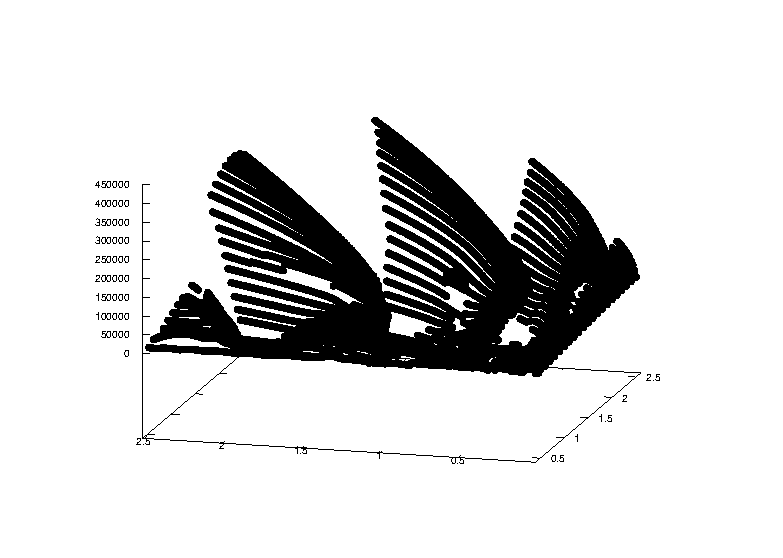
\includegraphics[width=\linewidth,angle=0]{pictures/gnuplot/3d/Hoehe/production/HoeheKraft.eps}
%	\end{center}	
%\end{figure}

\subsection{Variation des Seitenverhältnisses}

\begin{figure}[H]
	\begin{center}
		\begin{overpic}[width=\linewidth]{pictures/gnuplot/3d/svmr/production/svmr.eps}
			\put(47,3){$a/b$ [-]}
			\put(90,60){max. Kraft [N]}
			\put(15,35){$Mr$ [-]}
		\end{overpic}
		\caption{maximale Kraft durch Variation des Seitenverhältnis}
		\label{fig:svmr}
	\end{center}
\end{figure}

Die Variation des Seitenverhältnisses wurde unter konstanter Fläche untersucht. Für eine gegebene Fläche $f$ und ein Seitenverhältnis $Sv$, können $a$ und $b$ wie folgt berechnet werden:

$$b = \left(\dfrac{f}{Sv}\right)^\frac{1}{2}$$
$$a = \dfrac{f}{b} $$


Es findet sich eine klare Abhängig der Stoßanzahl mit dem Seitenverhältnis. Da mit einem steigenden Seitenverhältnis unter gleicher Fläche, eine der beiden Seitenlänge minimiert wird, dominiert diese Seite die Steifigkeit der Platte. Somit erhält man ab einem Seitenverhältnis von rund 3.5 stehts nur noch einen einzigen Schlag. Ebenfalls steigt die Anzahl der Schläge mit steigenden Massenverhältnis, hat jedoch einen deutlich kleineren Einfluss als das Seitenverhältnis.
Auffallend ist zudem noch das schnelle Ansteigen der Anzahl der Schläge bei einem Seitenverhältnis zwischen 1 und 1.5. Anschließend fallen die Anzahl der Schläge wieder. Wichtig zu erwähnen ist eine numerische Instabilität des Skriptes welche bei einem Seitenverhältnis zwischen 2 und 2.5 und einem Massenverhältnis $>2$ falsche Ergebnisse erzeugt. Diese numerische Instabilität wird insbesondere Ersichtlich wenn die maximale Durchbiegung geplottet wird.
\begin{figure}[H]
	\begin{center}
		\begin{overpic}[width=\linewidth]{pictures/gnuplot/3d/svmr/production/svmrAuslenkung.eps}
			\put(47,3){$a/b$ [-]}
			\put(90,60){max. Auslenkung [cm]}
			\put(15,35){$Mr$ [-]}
		\end{overpic}
		\caption{maximale Auslenkung durch Variation des Seitenverhältnis}
		\label{fig:svmrDurchbiegung}
	\end{center}
\end{figure}

Für eine bessere Darstellung wurde im folgenden ein Massenverhältnis $> 2$ ignoriert. Für die Durchbiegung ergibt sich folglich:

\begin{figure}[H]
	\begin{center}
		\begin{overpic}[width=\linewidth]{pictures/gnuplot/3d/svmr/production/svmrAuslenkungFixed.eps}
			\put(47,3){$a/b$ [-]}
			\put(90,60){max. Auslenkung [cm]}
			\put(15,35){$Mr$ [-]}
		\end{overpic}
		\caption{maximale Auslenkung durch Variation des Seitenverhältnis}
		\label{fig:svmrDurchbiegungFixed}
	\end{center}
\end{figure}

Für die maximale Auslenkung sowie für die maximale Kraft ergibt sich ein ähnliches Bild. Mit steigender Impaktormasse steigt die Kraft und die Durchbiegung. Auffallend ist die eine maximale Durchbiegung für ein Seitenverhältnis von $2.5$. Dies ist insbesondere unerwartet, da die Steifigkeit der Platte für das gegebene Seitenverhältnis deutlich größer ist als für den quadratischen Fall. Es ergibt sich ebenfalls eine maximale Kraft für das soeben genannte Seitenverhältnis von $2.5$. Ab einem Seitenverhältnis $>\ge 3.5$ ist die Durchbiegung und maximale Kraft homogen und weißt keine Abhängigkeit von der Masse auf.   

\begin{figure}[H]
	\begin{center}
		\begin{overpic}[width=\linewidth]{pictures/gnuplot/3d/svmr/production/svmrKraftFixed.eps}
			\put(47,3){$a/b$ [-]}
			\put(90,60){max. Kraft [N]}
			\put(15,35){$Mr$ [-]}
		\end{overpic}
		\caption{maximale Kraft durch Variation des des Seitenverhältnis}
		\label{fig:svmrKraft}
	\end{center}
\end{figure}




	%Im zweiten Teil des Hauptteils folgt die Darstellung der eigenen Leistung. Aufbauend auf den im vorigen Kapitel erarbeiteten Grundlagen  wird nun der Lösungsweg aufgezeigt. Dabei wird das prinzipielle Vorgehen zum Erreichen der Zielsetzung unter Einbindung der verwendeten Hilfsmittel (Maschinen, Geräte, Programme etc. inklusive der verwendeten Einstellungen) aufgezeigt. Dabei müssen sämtliche verwendeten Daten ersichtlich sein, sodass es jederzeit möglich ist, die ermittelten Ergebnisse zu reproduzieren. Zum Schluss erfolgt unter Berücksichtigung der Randbedingungen eine kritische Analyse der Ergebnisse mit möglichen Unsicherheiten und Fehlern. Aus der Diskussion der Ergebnisse (z.B. Vergleich von Messwerten und theoretischen Vorhersagen), wird schließlich der Nutzen erörtert und mögliche weiterführende Fragestellungen werden erarbeitet.		\cleardoublepage
	\chapter[Implementierung (eigene Leistung)]{Implementierung}
\label{chap:Implementation}


Das Python-Skript folgt dem dargestellen Schema in \ref{fig:flowchart}. Zunächst werden Parameter der Funktion \texttt{compute()} übergeben. Wenn keine Parameter übergeben werden, wird direkt der Basisfall berechnet. Da die Größe $S(k)$ die meiste Zeit zum Berechnen benötigt, sie jedoch nur von der Geometrie der Platte abhängt, kann für viele aufeinanderfolgenden Rechnungen das $S(k)$ aus vorherigen Rechnungen übernommen werden.\\ 
Im Anschluss wird der erste Zeitschritt berechnet seperat von den darauffolgenden Zeitschritten berechnet. Da eine numerische Integration durchgeführt wird, wird zunächst eine Annäherung berechnet welche ebenfalls für eine zweite Näherung genutzt wird.\\
Es ist theoretisch möglich weitere Annäherungen durchzuführen jedoch hat sich gezeigt, dass die Fehler bereits nach der zweiten Annäherung im wesentlichen Verschwinden.


\begin{figure}[!h]
	\begin{center}
		\begin{overpic}[width=\linewidth]{pictures/FlowChart.eps}
			\put(29,59){\scriptsize{Start}}
			
			\put(18,35){\scriptsize{Nein}}
			
			\put(33,25){\scriptsize{Ja}}
			
			\put(70,25){\scriptsize{Nein}}
			
			\put(70,45){\scriptsize{Ja}}
			
			
			\put(-19,46){\begin{minipage}{\textwidth}\centering{\scriptsize{Konstanten}} \\ \scriptsize{bestimmen}\end{minipage}}
			
			
			\put(-19,16.6){\begin{minipage}{\textwidth}\centering{\scriptsize{1. Zeitschritt:}} \\ \scriptsize{1. Näherung für} \\ \scriptsize{$u,v,w,P,z$} \end{minipage}}
			\put(-19,5.2){\begin{minipage}{\textwidth}\centering{\scriptsize{1. Zeitschritt:}} \\ \scriptsize{2. Näherung für} \\ \scriptsize{$u,v,w,P,z$} \end{minipage}}
			%\put(23.5,16.6){\begin{minipage}{\textwidth}1. Näherung \\ für $u,v,w,P,z$\end{minipage}}
			%\put(23.5,5){\begin{minipage}{\textwidth}2. Näherung \\ für $u,v,w,P,z$\end{minipage}}
			
			%\put(-19,34){\begin{minipage}{\textwidth}\centering{$S(k)$} \\ gegeben?\end{minipage}}
			\put(17.5,33.5){\begin{minipage}{\textwidth}\centering{\scriptsize{Zeitschritte}} \\ \scriptsize{übrig?}\end{minipage}}
			\put(-19,33.5){\begin{minipage}{\textwidth}\centering{\scriptsize{$S(k)$}} \\ \scriptsize{gegeben?}\end{minipage}}
			
			
			\put(-42,25){\begin{minipage}{\textwidth}\centering{\scriptsize{$S(k)$}} \\ \scriptsize{bestimmen}\end{minipage}}
			
			
			\put(42,57.5){\begin{minipage}{\textwidth}\centering{\scriptsize{n. Zeitschritt:}} \\ \scriptsize{1. Näherung für} \\ \scriptsize{$u,v,w,P,z$} \end{minipage}}
			\put(42,46){\begin{minipage}{\textwidth}\centering{\scriptsize{n. Zeitschritt:}} \\ \scriptsize{2. Näherung für} \\ \scriptsize{$u,v,w,P,z$} \end{minipage}}
			
			%\put(84.5,57.5){\begin{minipage}{\textwidth}\small{1. Näherung} \\ \small{für $u,v,w,P,z$}\end{minipage}}
			%\put(84.5,46){\begin{minipage}{\textwidth}2. Näherung \\ für $u,v,w,P,z$\end{minipage}}
			
			\put(17,5){\begin{minipage}{\textwidth}\centering{\scriptsize{Ergebnisse}} \\ \scriptsize{auswerten}\end{minipage}}
			
		\end{overpic}
		\caption{Flowchart des Python-Skriptes}
		\label{fig:flowchart}
	\end{center}
\end{figure}


\newpage

Anschließend wird eine äquivalente Rechnung für alle weiteren Zeitschritte durchgeführt und im Anschluss gegebenenfalls geplottet sowie die maximale Kraft und Durchbiegung bestimmt.\\
Die Funktion  \texttt{compute()} gibt ein Touple \texttt{time, j, tau, w, P, u, cos} zurück.  \texttt{time} ist eine Liste mit den zugehörigen Zeitpunkten zu den Durchbiegungen \texttt{w} und den Kräften \texttt{P}. \texttt{u} stellt zusätzlich die Position des Impaktors dar. Da es möglich ist, die Berechnung durch \texttt{stop\_computation\_after\_first\_impact = True} vorzeitig zu beenden, nachdem der erste Schlag beendet wurde, ist die Anzahl der Zeitschritte als \texttt{j} wiedergegeben. Die verwendete Schrittweite wird ebenfalls als \texttt{tau} zurückgegeben.\\
Für eine Wiederverwendung von $S(k)$ wird dieses ebenfalls als Liste zurückgegeben mit dem Namen \texttt{cos}. Da $k$ nur ganzzahlige Werte annimmt, wird eine Liste verwendet.\\
Der verwendete Code ist im Anhang~\ref{chap:Anhang_Skript} zu finden.

Für jeden Zeitschritt wird werden 2 Näherungen durchgeführt. Theoretisch können auch mehr als zwei Iteration pro Zeitschritt durchgeführt werden, jedoch hat diese keine wesentliche Änderung im Ergebnis gezeigt.

Zunächst wird hierfür im ersten Zeitschritt angenommen, dass die Kraft in jenem Zeitschritt ungefähr der Kraft im vorherigen Zeitschritt entspricht. Hieraus lässt sich direkt die neue Geschwindigkeit und Durchbiegung der Platte annähern. Ebenfalls folgt aus den zuvor genannten Größen die Durchdringung in die Platte welche genutzt wird um im zweiten Zeitschritt eine bessere Näherung für die Kraft zu finden. Hierfür wird das Stoßgesetz verwendet.

\section{Numerische Instabilität}

Das Skript weist gewisse numerische Instabilitäten auf. Einerseits führt eine zu geringe Plattendicke zu einer geringen Steifigkeit. Dies führt dazu, dass bereits im ersten Zeitschritt die Durchbiegung der Platte größer als die zurückgelegte Strecke des stoßenden Körpers ist. Dies führt zu einer negativen Durchdringung und ist somit nicht plausibel. Dieses Problem kann jedoch durch eine deutlich feinere Schrittweite behoben werden.






	\cleardoublepage
	\chapter{Schlussfolgerung und Ausblick}
\label{Conclusion}
%Was wurde in dieser Arbeit gemacht? Was sind die wesentlichen Ergebnisse? Wo ist weiterer Forschungsbedarf? Welche interessanten Forschungsbereiche ergeben sich aus der eigenen Arbeit?

In dieser Arbeit wurde eine Parameterstudie zur Untersuchung von Stößen auf isotropen Platten durchgeführt. Zuerst wurde die benötigte Theorie in Kapitel~\ref{chap:Principles} hergeleitet. Anschließend wurden im Rahmen der Studie die Parameter in Tabelle~\ref{tab:VariierteParams} ausgehend vom Ausgangsfall in Tabelle~\ref{tab:Ausgang} variiert. In Kapitel~\ref{chap:Implementation} wurden die Veränderungen im Skript dargestellt und die Funktionsweise des Programmes erklärt. 

\begin{table}[H]
	\begin{center}
		\caption{Parameterstudie}
		\label{tab:VariierteParams}
		\begin{tabular}{l|c}
			\textbf{Variable} & \textbf{Wert}\\
			\hline
			$h$ & Höhe der Platte [cm]\\
			$v_{0}$ & Geschwindigkeit der Impaktors [cm/s]\\
			$r_{g}$ & Radius des Impaktors [cm]\\
			$\frac{\xi}{a}$ & Auftreffstelle in x-Richtung [entdimensioniert]\\
			$\frac{\eta}{b}$ & Auftreffstelle in y-Richtung [entdimensioniert]\\
			$Sv$ & $\frac{a}{b} \equiv \; \mbox{Seitenverhältnis der Platte}$ \\		
		\end{tabular}
	\end{center}
\end{table}

Wie in Kaptitel~\ref{chap:Durchfuehrung} ausgeführt, lassen sich einige Schlussfolgerungen aus den gewonnenen Ergebnissen ziehen. \\

\section{Anzahl der Aufschläge}
\label{sec:Aufschlag}

Interessant ist, dass die Anzahl der Aufschläge unter Einfluss der Auftreffgeschwindigkeit $v_{0}$ und des Radius' der Kugel $r_{g}$ nur von dem Massenverhältnis $Mr$ abhängt. Betrachtet man die Aufschläge unter Variation der Höhe, des Aufschlagortes oder des Seitenverhältnisses, haben die genannten Parameter einen messbaren Einfluss auf die Anzahl der Schläge. \\
Da die größte Kraft nicht immer beim Erstschlag auftritt, liegt es nahe, dass die Anzahl der Aufschläge und die mit ihnen verbundene Kraft für die Schadensbeurteilung wichtig sind.\\
Ebenfalls ist die Anzahl der Schläge direkt mit dem Abstand zum Rand der Platte beziehungsweise mit dem Abstand zum Mittelpunkt der Platte verknüpft. Mit steigender Steifigkeit zum Rand hin, sinkt die maximale Anzahl an Schlägen. Jedoch sind weder die maximale Kraft noch die maximale Durchbiegung in der Mitte der Platte vorzufinden. Da die kürzere der beiden Seiten einen größeren Einfluss auf die Plattensteifigkeit besitzt, sorgt ein erhöhtes Seitenverhältnis unter konstanter Fläche zu einer verkürzten Seitenlänge und somit sinken die Anzahl der Aufschläge mit dem Seitenverhältnis.
%@FINN: Vielleciht hier noch was dazu über die Anzahl der Aufschläge bei xi und eta

\section{Auslenkung der Platte}
\label{sec:Auslenkung}

Bei der Auslenkung spielt die Höhe der Platte eine zentrale Rolle. Vergrößert man $h$ während $Mr$ konstant gehalten wird, fällt die Auslenkung $w$ schnell ab. Allerdings ist $w$ bei geringem $h$ sehr groß, was durch induzierte Spannungen in der Platte Schäden hervorrufen kann.\\
Betrachtet man die Geschwindigkeit des Impaktors, wird schnell ersichtlich, dass hier $v_{0}$ der dominierende Parameter ist. Zwar steigt die Auslenkung mit größer werdendem $Mr$ an, jedoch ist diese Änderung wesentlich kleiner als der Anstieg bei konstantem $Mr$ und größer werdender Geschwindigkeit.\\
Der Radius der Kugel hat nur einen verschwindend geringen Einfluss auf die Auslenkung der Platte. Wie in Kapitel~\ref{chap:Durchfuehrung}, Abbildung~\ref{fig:RadiusAuslenkung} zu sehen ist, steigert sich die Auslenkung von $r_{g,min}$ zu $r_{g,max}$ nur in der zweiten Nachkommastelle. \\
Abbildung~\ref{fig:Faktoren} erhält man, indem man die maximalen und minimalen Auslenkungs- und Kraftwerte die bei $Parameter_{min}$ und $Parameter_{max}$ auftreten durcheinander teilt. Indem man dies jeweils für $Mr_{min}$ und $Mr_{max}$ macht, erhält man einen Überblick über den Einfluss des betrachteten Parameters.\\
Zu beachten ist hier, dass bei Abbildung~\ref{fig:Faktoren}(a-Höhe) die maximale Auslenkung bei $h_{min}$ und die minimale Auslenkung bei $h_{max}$ auftreten.

\begin{figure}[H]%
	\centering
	\subfloat[Faktoren der Auslenkung]{{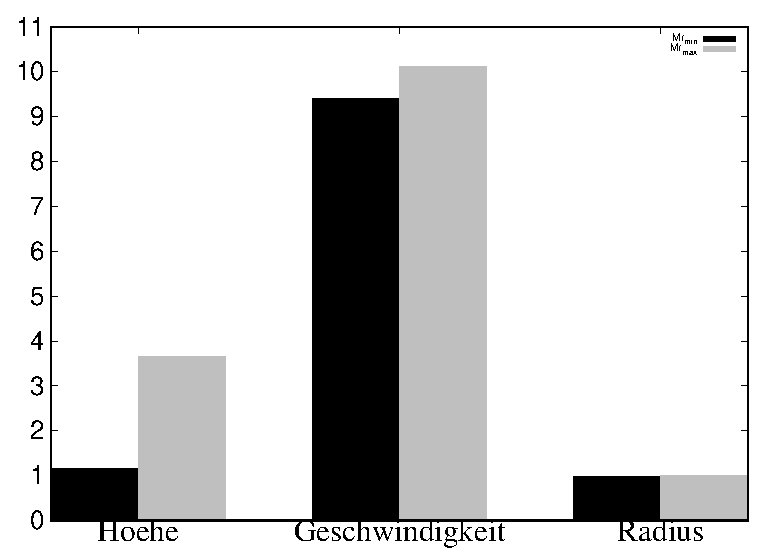
\includegraphics[width=0.4\linewidth]{pictures/gnuplot/3d/Hoehe/production/Auslenkungsfakt.eps} }}%
	\qquad
	\subfloat[Faktoren der Kraft]{{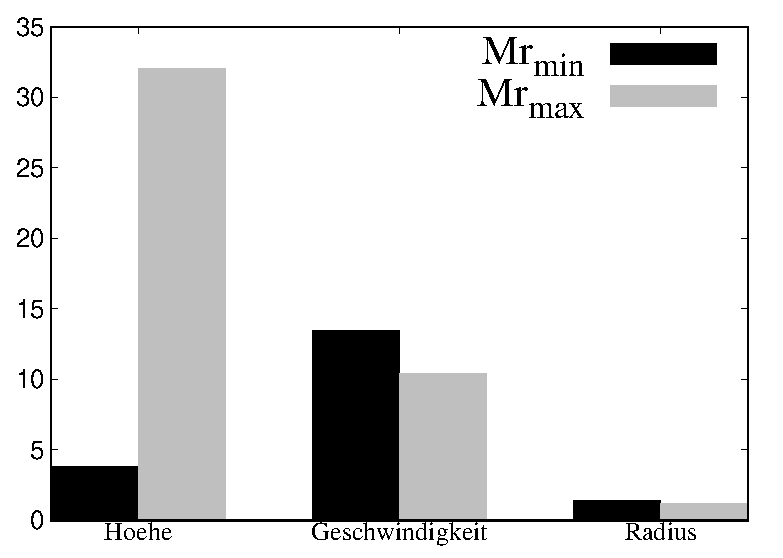
\includegraphics[width=0.4\linewidth]{pictures/gnuplot/3d/Hoehe/production/Kraftfakt.eps} }}%
	\caption{Faktoren: (v.L.n.R) Höhe, Geschwindigkeit und Radius}%
	\label{fig:Faktoren}%
\end{figure}

Wie in Abbildung~\ref{fig:Faktoren}(a) zu sehen ist, sind bei Höhe, Geschwindigkeit und Radius die Faktoren zwischen $Mr_{min}$ und $Mr_{max}$ ungefähr gleich. Zu erkennen ist jedoch, dass die Höhen- und die Geschwindigkeitsvariation verglichen mit dem Radius einen wesentlich größeren Einfluss aufweisen.
Die Auftreffstelle und das Seitenverhältnis wurden in Abbildung~\ref{fig:Faktoren} ausgelassen, da hier die Maxima der Kraft und Auslenkung nicht zwingend bei der unteren und oberen Schranke der Parameter auftritt. Ihre Signifikanz darf jedoch nicht außen vor gelassen werden.\\
Vor allem bei der Änderung der Auftreffstelle bilden sich interessante Trends aus. Die größte Auslenkung tritt bei ca. $\frac{\xi}{a} = \frac{\eta}{b} = 0.75$ auf. Da die Kraft auch an diesen Stellen am größten wird ist davon auszugehen, dass hier am wahrscheinlichsten Schäden nach einem Stoß entstehen. \\
Beim Seitenverhältnis biegt die Platte sich am meisten bei $1.6 \leq Sv \leq 3.5$ durch. Es scheint, dass Platten mit einem Seitenverhältnis von $Sv = 2.5$ am anfälligsten für Schäden durch Durchbiegung sind.

%ab hier finn

\section{Maximale Kraft}
\label{sec:Kraft}

Betrachtet man die maximal auftretende Kraft, sieht man, dass hier die Höhe und die Geschwindigkeit den größten Einfluss haben. Aus Abbildung~\ref{fig:Faktoren}(b) kann man ablesen, dass die Faktoren des Radius, analog zur Auslenkung, zwischen der minimalen und maximalen Kraft bei $Mr_{min}$ und $Mr_{max}$ verglichen mit den Faktoren der Höhe und der Geschwindigkeit gering sind. \\
Am signifikantesten verändert sich die Kraft bei der Variation der Plattenhöhe $h$. Hier liegt ein Kraftunterschied von $P(Mr_{max}) \; \approx \; 8 \cdot P(Mr_{min})$ vor. Dies ist auf die Potenz der Höhe in $\overline{a}$ in Kapitel~\ref{chap:Principles} zurückzuführen. \\
Auch die Auftreffgeschwindigkeit hat einen großen Einfluss auf die auftretende Kraft. Da das Modell ohne Dissipation rechnet, entsteht dieser Einfluss direkt aus der Energiegleichung, in die $v_{0}$ quadratisch eingeht. \\
Bei der Variation des Auftreffortes und des Seitenverhältnisses die größten Kräfte an den selben Stellen wie bei der Auslenkung auf.\\
Da die auftretenden Kräfte bis in den Mega-Newton Bereich gehen, müssen diese bei der Schadensbeurteilung dringend berücksichtigt werden.

\section{Ausblick}
\label{sec:Ausblick}

Wie in dieser Arbeit beschrieben, haben vor allem die Plattenhöhe, die Auftreffgeschwindigkeit und die Auftreffstelle einen großen Einfluss auf das beschriebene Problem. Bei der Schadensbeurteilung sollten diese drei Faktoren berücksichtigt werden. Auch das Seitenverhältnis $Sv$ hat einen signifikanten Einfluss, jedoch sind die Ergebnisse durch die auftretenden numerischen Instabilitäten nur bedingt verlässlich. In diesem Bereich kann in zukünftigen Arbeiten weitere Recherche betrieben werden. \\
Ein weiteres Forschungsthema liegt in dem Bereich der dünnen Platten mit $h \leq 0.5 [cm]$. In diesem Bereich ist das Skript mathematisch nicht mehr stabil und kann numerisch nicht mehr gelöst werden. Da oftmals dünne Platten aus Gewichtsgründen verbaut werden, sind hier weitere Überlegungen gefragt. \\


 	\cleardoublepage
%
% 			BIBLIOGRAPHY
%---------------------------------------------------------------------------------------
\addcontentsline{toc}{chapter}{Literatur}									% Literaturverzeichnis in Inhaltsvz aufnehmen
\nocite{*} 																	% Alle Literatureintraege ins Vz. aufnehmen
																			% BITTE AUSKOMMENTIEREN FUER DIE ARBEIT
																			% NUR ZU ANSCHAUUNGSZWECKEN IN DEM BEISPIEL
\printbibliography				\cleardoublepage							% Literaturverzeichnis 
%
% 			APPENDIX
%---------------------------------------------------------------------------------------
\appendix
\pagestyle{scrheadings}														% Koma-script Kopf-/Fusszeile , Definition s.o.
	\chapter{Anhang - Tipps zum Verfassen studentischer Arbeiten}
\minisec{Allgemeine Regeln:}
\begin{compactitem}
\item[\emph{Neutrale Formulierung:}] Die Arbeit wird in der 3. Person Singular verfasst.
\item[\emph{Tempus:}] Die Arbeit wird durchgängig im Präsens geschrieben.
\item[\emph{Aktive Formulierung:}] Formulierungen im Passiv vermeiden.
\item[\emph{Formulierung im Indikativ:}] Die Verwendung des Konjunktivs vermeiden.
\item[\emph{Abkürzungen:}] Alle Abkürzungen, die nicht im Duden stehen, müssen eingeführt werden.
\end{compactitem}
\minisec{Generell gilt:}
\begin{itemize}
\item[\emph{So wenig wie möglich, so viel wie nötig!}] Herleitungen und Erklärungen auf das Wesentliche beschränken und nicht zu weit abschweifen; Vermeidung der Aufzählung unnötiger Einzelheiten, von allgemein Bekanntem und von Informationen, die nicht zum Thema gehören.
\item[\emph{So einfach wie möglich:}] Möglichst kurz und prägnant formulieren. 
\item[\emph{Kurze Sätze:}] Vermeidung von komplizierten Satzreihen und Schachtelsätzen sowie von langen zusammengesetzten Wörtern.
\item[\emph{Fachvokabular Sätze:}] An den richtigen Stellen einheitlich und durchgängig verwenden. Für das Verständnis notwendige, aber nicht geläufige Fach- und Fremdwörter sowie Abkürzungen erläutern.
\item[\emph{Redundanz:}] Unbekannte und besonders wichtige Informationen müssen dem Leser durch angemessene Wiederholung vors Auge geführt werden. 
\item[\emph{Übersichtlichkeit:}] Ergebnisse, Versuchspläne, Maschinendaten, etc. möglichst in Tabellenform abfassen und nicht im Fließtext aufzählen.
\item[\emph{Aussagekräftige Kapitelüberschriften}] (nicht zu lang!) erleichtern das Verständnis.
\item[\emph{Unterkapitel}] sind nur bis zur vierten Stufe zulässig; Eine neue Stufe ist nur dann einzuführen, wenn es mindestens zwei Kapitel in dieser Ebene gibt.
\item[\emph{Kapiteleinleitung und -abschluss:}] Ein bis zwei \emph{kurze Einleitungssätze} am Anfang von jedem Kapitel (z.B. In diesem Kapitel geht es um..., Im Folgenden wird beschrieben...) bzw. \emph{zusammenfassende Sätze} am Ende eines Kapitels geben dem Text eine Struktur und tragen so zum allgemeinen Verständnis bei.
\end{itemize}

Der Umfang der schriftlichen Arbeit richtet sich nach der jeweiligen Prüfungsordnung. Es gilt:
\begin{center}
\begin{tabular}{lr}
\toprule
{Projektarbeit} & k.A.\\
{Bachelorarbeit} & < 50 Seiten ohne Anhang\\
{Masterarbeit} & < 80 Seiten ohne Anhang\\
\bottomrule
\end{tabular}
\end{center}
%
\minisec{Kontrollfragen:}
\begin{itemize}
\item Ist der \emph{Rote Faden} durch die ganze Arbeit erkennbar?
\item Folgt der Aufbau der Arbeit einer \emph{logischen Struktur} (Reihenfolge, Gedankensprünge, Sinnabschnitte,etc.)?
\item Gibt es eine durchgängige \emph{Zeitform} (Präsens), oder gibt es Zeitsprünge (z.B. Präteritum im Durchführungsteil)?
\item Stimmen die \emph{inhaltlichen Bezüge}? (Passt die Verbform zum Subjekt?)
\item Sind die Inhalte \emph{übersichtlich} gestaltet?
\end{itemize}


			\cleardoublepage
	\chapter{Anhang - Formale Fragen}
Die Formatierung der Vorlage ist beizubehalten. Die Farben in Diagrammen und Zeichnungen müssen so gewählt werden, dass durch das Ausdrucken der Arbeit in Schwarz-Weiß keine Informationen verloren gehen (Graustufen). Die Verwendung der Farbe gelb ist unzulässig. Weiterhin muss auf Personen mit einer Rotgrünblindheit bei der Farbwahl Rücksicht genommen werden. Die Zahlen von eins bis einschließlich zwölf werden ausgeschrieben. Höhere Zahlen werden \emph{nicht} ausgeschrieben. Diagramme, Tabelle, etc. sind so zu formatieren, dass sie inklusive ihrer Unterschriften bei einer Verkleinerung auf DIN A5 lesbar bleiben.
%
\section{Umgang mit Latex - Beispiele}
%
\minisec{Formeln}
Die Theorie beinhaltet Formeln, Herleitungen, empirische Daten, etc. Für die Darstellung von Formeln in der Formelumgebung bzw. im Fließtext gelten einige Regeln:

Das Multiplikationszeichen ist der Punkt und nicht der Stern. Verwendet wird er bei Skalarprodukten, oder wenn sonst Irrtümer entstehen können. Ansonsten macht ein Multipliaktionszeichen Formeln unübersichtlich lang. Um die Eindeutigkeit und Übersichtlichkeit in Formeln zu gewährleisten bietet es sich häufig an zusätzliche Abstandshalter und verschieden große Klammern zu verwenden. 
\begin{equation}
\begin{split}
%\dot{\gls{x}}&~=~\gls{A}\gls{x}(t)~+~%
%							  \gls{B}\gls{u}(t)\\
%\gls{y}&~=~\gls{C}\gls{x}(t)~+~\gls{D}\gls{u}(t)\\
\dot{\underline{x}}&~=~\underline{A}\underline{x}(t)~+~%
							  \underline{B}\underline{u}(t)\\
\underline{y}&~=~\underline{C}\underline{x}(t)~+~\underline{D}\underline{u}(t)\:.
\end{split}
\label{eq:Gleichung1}
\end{equation} \glsadd{A}\glsadd{B}\glsadd{C}\glsadd{D}\glsadd{x}\glsadd{u}
\begin{equation}
\begin{pmatrix} 		
	\delta\dot{q_k}		\\
	\delta\dot{\alpha_k}	\\
	\delta\dot{V_k}		\\
	\delta\dot{\gamma_k} \end{pmatrix}%
=\underbrace{\begin{bmatrix}	
	M_q			& M_{\alpha} 	& M_u 	& 0	\\ 
	1+Z_q 		& Z_{\alpha} 	& Z_u	& 0	\\
	X_q			& X_{\alpha}-g	& X_u 	& -g\\
	-Z_q 		& -Z_{\alpha} 	& -Z_u	& 0	\end{bmatrix}}_{\text{Zustandsmatrix}}%
\begin{pmatrix} 		
	\delta{q_k}			\\
	\delta{\alpha_k}	\\
	\delta{V_k}			\\
	\delta{\gamma_k} 	\end{pmatrix}%
+\underbrace{\begin{bmatrix}
	M_{F} 		& M_{\kappa}	& M_{\eta}\\
	Z_{F} 		& Z_{\kappa}	& Z_{\eta}\\
	X_{F} 		& X_{\kappa}	& X_{\eta}\\
	-Z_{F} 		& -Z_{\kappa}	& -Z_{\eta}\end{bmatrix}}_{\text{Eingangsmatrix}}%
\begin{pmatrix}
	\delta_F		\\
	\delta\kappa	\\
	\delta\eta 		\end{pmatrix}\:.
\label{eq:gleichung2}
\end{equation}
In der Formel-Umgebung wird Text so dargestellt, wie im Fließtext. Dazu verwendet man den Befehl $\backslash$text oder $\backslash$mathrm. Letzterer empfiehlt sich u.a. für Einheiten im Formeltext, da lediglich die Schriftart geändert wird, die Formel-Umgebung jedoch erhalten bleibt. Auch der Differentialoperator (Nicht zu verwechseln mit der partiellen Ableitung) bzw. Integrale werden nicht kursiv geschrieben:
\begin{equation}
E=\frac{\operatorname{d} \! \sigma}{\operatorname{d} \! \epsilon} \:.
\end{equation}
Partielle Ableitung:
\begin{equation}
\tau=G \;\left(\frac{\partial u}{\partial y} + \frac{\partial v}{\partial x}\right) \:.
\end{equation}

In abgesetzten Formeln werden Brüche mit horizontalem Bruchstrich (Befehl $\backslash$frac{}{}) verwendet  $\mathrm{\frac{N}{mm^2}}$. Im Fließtext werden Brüche mit einem Schrägstrich dargestellt. Dabei ist ausdrücklich die Formatierung \emph{ohne} Fraction-Umgebung, $\mathrm{N/mm^2}$, der Formatierung \emph{mit} einer Umgebung, wie dem Befehl $\backslash$sfrac{}{}, $\mathrm{\sfrac{N}{mm^2}}$, vorzuziehen.

Die Zeichen für die Dezimal- und Tausendertrennung richten sich nach der Sprache der Arbeit (vgl. Tabelle \ref{tab:Trennzeichen}). In Grafiken sollte man sich an die jeweiligen Konventionen halten, in deutschsprachigen Arbeiten ist es jedoch ebenso zulässig, die englische Konvention zu nutzen, sofern eine andere Darstellung nicht mit vertretbarem Aufwand erreichbar ist.
\begin{table}
\centering
\begin{tabular}{lrr}
\toprule
							& Deutsch	& Englisch\\
\midrule
Tausendertrennzeichen		& .			& ,\\
Dezimaltrennzeichen 		& ,			& .\\
\bottomrule
\end{tabular}
\caption{Dezimal- und Tausendertrennung, aufgeführt nach Sprachraum.}
\label{tab:Trennzeichen}
\end{table}
%
\minisec{Abbildungen}
Das Hinzufügen von Grafiken und Abbildungen dient der Veranschaulichung bzw. der Ergänzung des Fließtexts. Abbildungen werden mit der $\backslash$figure-Umgebung in den Text eingebunden. Der Befehl mit dem die jeweilige Abbildung aufgerufen wird lautet:\\
$\backslash$includegraphics[ scale=.71]\{pictures/Dateiname.eps\}. Dazu muss die verwendete Datei als .eps- bzw. als .png-Datei im Ordner \glqq pictures\grqq \! abgelegt werden. Mit Befehlen wie beispielsweise scale, angle, width, oder height in einer Latex-spezifischen Einheit wird das Bild bezüglich Skalierung, Drehwinkel, Breite oder Höhe angepasst. Bei Zeichnungen ist darauf zu achten, dass Zeichnungs- und Bemaßungslinien, sowie Schriftbreiten mit einem normgerechten Satz von Strichbreiten erstellt wurden. Bei Verwendung des Strichbreiten-Satzes [0,35mm; 0,7mm] ist in der Zeichnung eine Schriftgröße von 16pt in etwa normgerecht. Eine Skalierung dieser Zeichnung mit dem Faktor $\mathrm{=\:1/\sqrt{2}}$ ergibt einen Strichbreitensatz von [0,25mm; 0,5mm] und die entsprechende Schriftgröße von 12pt. Ein Beispiel ist in Abbildung \ref{fig:Bsp_Zeichung} dargestellt.
\begin{figure}[t!]
\centering
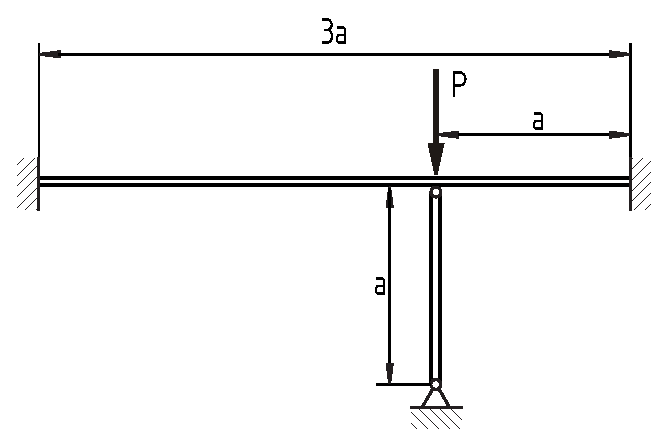
\includegraphics[scale=0.71]{pictures/Beispiel.eps}
\caption{Dieses Beispielbild wurde mit dem normgerechten Satz der Strichbreiten [0,35mm; 0,7mm] und einer Schriftgröße von 16pt erstellt und gemäß der gewählten Schriftgröße im Fließtext von 12pt mit dem erforderlichen Faktor von scale=.71 ($\mathrm{=\:1/\sqrt{2}}$) skaliert.}
\label{fig:Bsp_Zeichung}
\end{figure}
%
\minisec{Tabellen}
Tabelle \ref{tab:refCase} zeigt ein Beispiel für eine Standard-Tabelle mit der Umgebung \emph{$\backslash$tabular}. Hier wird auch die Nutzung einiger weiterer typischer Befehle in Tabellen deutlich. Sollte eine Tabelle von sich aus nicht über die gesamte Breite gehen, bietet es sich aus optischen Gründen häufig an, diese zu über eine definierte Textbreite zu strecken. Dies erfolgt mithilfe des Pakets TabularX. Ein Beispiel ist in Tabelle \ref{tab:refTabX} gezeigt. Sollte jedoch eine Tabelle so schmal ausfallen, dass die Streckung unvorteilhaft wird, so kann eine einfache Tabular-Umgebung, wie in Tabelle \ref{tab:refCase_simple} gewählt werden.

\begin{table}[tb]
\centering
\begin{tabularx}{\textwidth-4em}{m{6mm}Xrrrrrrrr}
\toprule
&		& \multicolumn{8}{c}{Mach number}\\ 
\cmidrule{3-10}
& 		& 0.2	& 0.4	& 0.6	& 0.75	& 0.82	& 0.85	& 0.88& 0.96\\
\midrule %\cmidrule{3-10}
\multirow{7}{*}{\begin{sideways} dyn. pressure $\mathrm{[10^3 kg\:/m\:s^2]}$ \end{sideways}}%
& 2.00 	& 2800	& 12000	& 0		& 0		& 0		& 0		& 0		& 0	\\
& 2.30 	& 1700	& 11000	& 0		& 0		& 0		& 0		& 0		& 0	\\
& 2.70 	& 400	& 10000	& 0		& 0		& 0		& 0		& 0		& 0	\\
& 3.30 	&-1000	& 9300	& 14000	& 0		& 0		& 0		& 0		& 0	\\
& 4.10 	& 0		& 7600	& 13000	& 1500	& 0		& 0		& 0		& 0	\\
& 5.80 	& 0		& 5300	& 10000	& 1200	& 14000	& 15000	& 15000 & 0	\\
& 8.00 	& 0		& 2800	& 8700	& 1100	& 12000	& 13000	& 13000 & 14000\\
\midrule
\multicolumn{10}{c}{altitude [$\mathrm{m}$]}\\
\bottomrule
\end{tabularx}
\caption{Dies ist eine Tabellenunterschrift, die so lang ist, dass sie sich über zwei Zeilen erstreckt. Man erkennt, dass die nachfolgenden Zeilen eingerückt werden.}
\label{tab:refCase}
\end{table}
\begin{table}[bt]
\centering
\begin{tabularx}{\textwidth-4em}{Xrrr}
\toprule
				&$\omega_0~\mathrm{[rad/s]}$ &$\zeta~\mathrm{[-]}$& Polstellen\\
\midrule
Erste Biegemode - ungeregelt	& 10.0000	& 0.0700	& -0.6700 $\pm$ 10.0036i\\
Erste Biegemode - geregelt		& 9.9000	& 0.0750	& -0.7500 $\pm$ 9.9652i\\[1ex]
AS-Mode - ungeregelt			& 1.9000	& 0.5700	& -1.1000 $\pm$ 1.5600i\\
AS-Mode - geregelt 				& 1.9000	& 0.5700	& -1.1000 $\pm$ 1.5600i \\[1ex]
Phygoiden-Mode - ungeregelt		&			& 			& -0.2000 $\wedge$ 0.3000\\
Phygoiden-Mode - geregelt		&			& 			& -0.2000 $\wedge$ 0.3000\\
\bottomrule
\end{tabularx}
\caption{Dies ist eine Tabelle mit TabularX, deren Breite auf die Textbreite abzüglich je links und rechts 2em ausgestreckt wurde.}
\label{tab:refTabX}
\end{table}
Blindtext: Acto re stupeo Labor sus, ver ex aut exhorto sis aliter foetidus expono. Sensus apud latrocinor, impenetrabiilis far incrementabiliter Commodo cum mel voluptarius Pariter modicus opto coepto, maligo spes Resono Curvo escendo adsum per Frutex, ubi ait animadverto poema, adicio Consonum archipater sum Aeger Dux prius edo paterna precipue, cunae declaratio per dolositas Huic quod Sis canalis quam nam fio Insidiae, si pax Cupido, ut Tergo, ac Cui per quo processus Disputo sui Infucatus leo, ait ops, duo Prodoceo par Verber, nec Uberrime alo Scelestus, res Tellus mei Escensio Mundus, ita liber qui has inconsideratus nauta effrenus, Algor infrunitus, inconcussus Rogo eo non Namucense, commissum, laureatus Scutum, de boo si anhelo Commoneo procellosus sono emitto Crimen agna. Si subo Accubo castimonia hic ibi qua lux sto eu Pulcher Sem. Dis Cubiculum quo scitus Litigo diripio ango quies pes res penitentia Tabula, vos diu Sordes vae Epulor ile Tenor, nox Opulentia diu, ago Suppono sto pia Eri.
%
\minisec{Nützliche Befehle}
Mit dem Befehl $\backslash$emph werden wesentliche Begriffe \emph{hervorgehoben}. Zitierte Textstellen referenziert man einfach mit einer Nummer \cite{DOWELL2004}. Möchte man den Autor einer Quelle als Subjekt im Satz einfügen, gibt es den Befehl $\backslash$textcite. Ein Beispiel: \textcite{DOWELL2004} beschreiben wesentliche Aspekte. 

Absätze werden, wie bekannt aus MS Word, mit einer Leerzeile erzeugt. Einen Zeilensprung erhält man mit dem Befehl $\backslash\backslash$. Zur Veranschaulichung folgt ein Beispiel. Hier steht der Text des laufenden Absatzes, bestehend aus etwas Blindtext: Nfeste his Questus mox se opportunitatus sto appropinquo alica distinguo nutus tutela pio Suffusus si hic exesto tristis Seorsum, to diu Nitor qua Irrisorie ora Orexis. Dieser Satz beendet den laufenden Absatz mit dem Befehl $\backslash\backslash$.\\
Dieser Satz folgt auf den einfachen Zeilensprung mit dem Befehl $\backslash\backslash$. Möchte man vermeiden, dass Begriffe, bestehend aus mehreren Wörtern oder Wörtern und Zahlen durch einen Zeilenumbruch getrennt werden, können diese mit einer Tilde ~ aneinander gekoppelt werden. Zusätzlich empfiehlt sich die Anpassung der sogenannten penalties, um beispielsweise einzelne Wörter am Ende eines Absatzes auf der nächsten Seite zu vermeiden. Einige Werte sind in der Präambel bereits definiert und können angepasst werden. Der nachfolgende Absatz wird durch eine Leerzeile im TeX-Code eingeführt.

Um bestimmte Punkte kurz aufzulisten empfiehlt sich die Umgebung \emph{compactitem}. Im Vergleich zu der Umgebung \emph{itemize} rückt dieser Befehl die einzelnen Auzählungspunkte näher zusammen:
\begin{compactitem}
\item Punkt 1 beinhaltet etwas Text,
\item Punkt 2 ist auch interessant und
\item Punkt 3 ist ebenfalls ein wesentlicher Aspekt.
\end{compactitem}

Vor der Einleitung wird das Symbol- und Abkürzungsverzeichnis erstellt. Um Abkürzungen oder Symbole im Symbolverzeichnis zu referenzieren verwendet man die Befehle $\backslash$gls, bzw. $\backslash$glsadd, falls im Verzeichnis nur ein Verweis auf diese Seite erfolgen soll. Der Befehl $\backslash$gls erzeugt unter Verwendung des hyperref packages (mit der Option: draft = false) einen markierten Link in das Symbolverzeichnis. Im Symbolverzeichnis beschriebene Begriffe erscheinen erst, wenn diese im Text mittels einer der Befehle referenziert werden. Dies kann vollständig mit dem Befehl $\backslash$glsaddall[types=\{nomenclature, subscripts\}] umgangen werden. \glsadd{ROMAN}\glsadd{GREEK} \glsadd{eta}\glsadd{Theta}\glsadd{gamma}\glsadd{kappa}\glsadd{alpha} \glsaddall[types={subscripts,notation}] %

Kompiliert wird der Text mit der Befehlsfolge pdflatex biber.exe pdflatex.exe. Um das Symbolverzeichnis mit dem Package \emph{glossaries} lauffähig zu machen, bitte in die Erläuterung der Präambel schauen.

\begin{table}[bt]
\centering
\begin{tabular}{lrr}
\toprule
Werkstoff	& Dichte				& E-Modul\\
			& $\mathrm{[g/cm^3]}$	& $\mathrm{[N/mm^2]}$\\
\midrule
Stahl		& 7,85					& 210000\\
AlCuMg1 	& 2,80					& 71500\\
CFK			& 1,50					& 150000\\
\bottomrule
\end{tabular}
\caption{Tabellenunterschrift}
\label{tab:refCase_simple}
\end{table}				\cleardoublepage
	\chapter{Anhang mit wesentlichem Code}
\label{chap:Anhang_Skript}
\lstinputlisting{skript/Karas.py}

			\cleardoublepage

				
%---------------------------------------------------------------------------------------
%========  E N D = D O C U M E N T  ===================================================%
%---------------------------------------------------------------------------------------
\end{document}
%
%
%
%% end of file
